% siminos/spatiotemp/chapter/Ising.tex
% $Author: predrag $ $Date: 2021-12-08 00:39:15 -0500 (Wed, 08 Dec 2021) $

\chapter{Ising model in 2D}
\label{chap:Ising2D}

\begin{bartlett}{
\toChaosBook{Item.258}
{\bf Exercise 17.1 Time reversibility.}
%\tangent
Hamiltonian flows are time reversible. Does that mean that
their \markGraph s are symmetric in all node$~\to~$node links,
their transition matrices are adjacency matrices, symmetric and
diagonalizable, and that they have only real eigenvalues?
%\label{e-TimRevrs}

Solution 14.1, 2021-12-07 Read \refsect{s:latt1d} and on for a
group-theoretic solution.
                }\bauthor{
An open exercise from ChaosBook.org
                }
\end{bartlett}

\bigskip

\begin{description}

    \PCpost{2016-02-19}{                    \toCB
A wild idea, to keep in mind, if we get to the point where QFT is within
reach.
`Fundamental domain' appears in an interesting stat mech context in Wipf
\etal\rf{WKWTP06,WHKW07} {\em Generalized {Potts-models} and their
relevance for gauge theories}. They study the 3-state Potts model, a
natural extension of the Ising model with 3 vectors at each site, whose
global symmetries are point group \Cn{3}, and the 1d lattice of discrete
translations. The domain of the traced Polyakov loop variable (?) for
\SUn{3} is a triangle, with a  \Cn{3} fundamental domain. Then they
compute leading terms in the strong coupling limit using characters
$\chi_{pq}$ for the \SUn{3} representation $(p,q)$. These characters
transform under \Cn{3}, so they restrict calculations to the fundamental
domain inside the above triangle. Or perhaps \Dn{3}, could not tell in my
first, very superficial reading. These articles were immediately followed
up by a bunch of other articles - there are too many quantum field
theorists out there:)

In other words, Potts model could provide a bridge from Boris' cat maps to
QFT on lattices.

There is also a continuation with $G_2$ Yang-Mills by the same authors,
but that's for another, more ambitious time...
   }

    \PCpost{2016-10-03}{
Not quick or easy to explain, but I have a hunch that the spatiotemporal
zeta function should be something like the 2D Ising model zeta function
described by Aizenman \HREF{160913IsingZeta.pdf} {(click here)}. It
should assign a weight for every spatiotemporal domain, described by its
2D symbolic dynamics.
    }

    \PCpost{2016-10-08}{
qmath16 Aizenman talk notes (mostly gibberish - my fault):

It is known (?) that QM is emergent from the \emph{classical} stat mech
of Ising models. Key tools: Pfaffians. Random current representation of
Ising.

Groenevald-Boel-Kasteleyn'78: describe correlations in the planar Ising
model, by boundary segments, ordered cyclically. Pfaffian refers to
spin-spin correlations along the boundary. There is a parity sign that
makes it a non-interacting fermion model.

Aizenman et al. extend it to nonplanar modles, where planarity
\emph{emerges} at the critical point. ADTW'16 proof utilizes the
\emph{random current representation}. Starts with high temperature
expansion. Partition function is a sum over loops. In a correlation,
sources are connected pairwise by lines, ie, Gaussian limit. Above
critical dimension - four - the theory is free (sum of products over
pairs). In 2D, fermionic case, you get Pfaffian. Leads to the
integrability of the model. (Read Chelkak-Cimasoni-Kassel '15.)

``Almost planar"

Order-disorder variables.

Aizenman: Two implications of planarity

1) For any planar graph, and a symmetric edge function
\[
{\cal F}(\{K_\theta\}) = \det(1-K{\cal W})
\]
is the \emph{square of a multilinear function} of the parameters
\(
\{K_\theta\}_{\theta \in \epsilon_0}
\,.
\)
This is proven through a reduction to an antisymmetric matrix $A$, and
(Kasteleyn matrix '63):
\[
\det (A) = \mbox{Pf}[A]^2.
\]


For planar models, done by Kac-Ward. Works for any planar graph
(``amorphous graphs''), not only on a regular lattice.

2) For any planar loop of oriented non-backtracking edges
\(
\{e_1, e_2, \cdots\}
\)
\[
\prod_{j=1}^n {\cal W}_{e_{j+1},e_j} = (-1)^{w(\rho^*)}
             = (-1)^{n(\rho^*)}
             \,.
\]
with $w(\rho^*) =$ winding number, and $n(\rho^*) = \#$~of {self
crossings } [Whitney's Thm].

This is then combined with the \emph{Ihara relation}, for matrices indexed by
oriented edges:
\[
\det(1- KW)_{\epsilon_0\times\epsilon_0}
= \prod_{\ell}\left[
            1+(-1)^{n(\ell)} \chi_{-K}(\ell)
            \right]^2.
\]
the product being over unoriented loops on $\mathbb{G}$ (hence the power 2).
    }

\item[2020-09-30 Predrag].

\videoLink{YouTube.com/%
watch?v=A_Jhee-s8jk} {Michael Aizenman biographical sketch}

Aizenman Rutgers talk (unrecorded) was a modal of clear exposition.
It is an audience
friendly explanation of the background to, and advance for $d=4$
explained in Michael Aizenman and Hugo Duminil-Copin {\em Marginal
triviality of the scaling limits of critical 4D Ising and $\phi_4^4$
models}, \arXiv{1912.07973}. Duminil-Copin will give a tutorial on this
work on October 9-10, 2020, in
\HREF{http://sites.math.northwestern.edu/mwp/}
{42nd Midwest Probability Colloquium}.

I especially liked the `reminder' explaining how $\phi^4$ goes to Ising in
particular limit.

Related publications to check:

Michael Aizenman and Simone Warzel {\em Kac-Ward formula and its
extension to order-disorder correlators through a graph zeta function},
\arXiv{1709.06052}
% doi 10.1007/s10955-018-2184-9

Is the \emph{loop-soup expansion} related to my random walk
interpretation of the hypercubic {\jacobianOrb} traces and the
determinant? References might be in Michael Aizenman, Hugo Duminil-Copin
and Simone Warzel {\em Dimerization and N{\'e}el order in different
quantum spin chains through a shared loop representation},
\arXiv{2002.02543}.
% doi 10.1007/s00023-020-00924-2

    \PCpost{2016-10-05}{
Aizenman, La{\'{\i}}nz Valc{\'a}zar and Warzel\rf{AiLVWa16}
{\em Pfaffian correlation functions of planar dimer covers}
does not seem to be what we need (no word `zeta' in this paper). They
refer to 2016 preprint  of

M. Aizenman H. Duminil-Copin, V. Tassion, S. Warzel,
{\em Fermionic correlation functions and emergent planarity in 2D Ising models}.
(that paper does not seem to be available anywhere, as yet)

The structure of the solution of Kac and Ward has been explained  in
unpublished lectures by Feynman (Aizenman referred to Feynman's stat mech
book).

Sherman\rf{Sherman60} {\em Combinatorial aspects of the {Ising} model for
ferromagnetism. {I. A} conjecture of {Feynman} on paths and graphs}

Hurst and Green\rf{HurGre60}
{\em New solution of the {Ising} problem for a rectangular lattice}

Burgoyne\rf{Burgoyne63}
{\em Remarks on the combinatorial approach to the Ising problem}

Vdovichenko\rf{Vdov65}
{\em A calculation of the partition function for a plane dipole lattice}.
The steps: a) the sum over polygons is reduced to a sum over closed
loops without intersections; b) the sum over closed loops without
intersections is transformed into a sum over all loops; c) the sum over
all loops is reduced to a random-walk problem and is calculated easily.

Cimasoni\rf{Cimasoni10}
{\em A generalized  {Kac-Ward} formula}: ``
As a consequence of our second proof, we also obtain the following fact:
the Kac–Ward and the Fisher–Kasteleyn methods for solving the Ising model
are one and the same.
''

Cimasoni\rf{Cimasoni12}
{\em The critical {Ising} model via {Kac-Ward} matrices}:
The Kac-Ward formula\rf{KacWar52} allows to compute the Ising partition
function on any finite graph G from a determinant with quite remarkable
properties. First of all, they satisfy some generalized Kramers-Wannier
duality: there is an explicit equality relating the determinants
associated to a graph and to its dual graph. Also, they are proportional
to the determinants of the discrete critical Laplacians on the graph G.

Fisher\rf{Fisher66}
{\em On the dimer solution of planar Ising models}

Kasteleyn\rf{Kasteleyn61}
{\em The statistics of dimers on a lattice:
    {I. The} number of dimer arrangements on a quadratic lattice}

Kasteleyn\rf{Kasteleyn63}
{\em Dimer statistics and phase transitions}

H.  Au-Yang,  J.  H.  H.  Perk.  Ising  correlations  at  the  critical  temperature.
Physics Letters A 104, 131–134 (1984).

Kager, Lis and Meester\rf{KaLiMe13}
{\em The  signed  loop  approach  to  the  Ising  model:
Foundations and critical point}

Lis\rf{Lis15}
{\em A short proof of the {Kac-Ward} formula}:
\beq
\det(Id-\Lambda)=\integers^2
\ee{Kac-Ward}
The original proof of Kac and Ward\rf{KacWar52} famously contained an
error. We refer the reader to \refref{KaLiMe13} for a longer discussion
on the history of this theorem. The main improvement here, in comparison
with \refref{KaLiMe13},  is that there is no need for expanding the
generating functions into generating functions of collections of loops.
The combinatorial mechanism of the Kac-Ward formula is here as
transparent as the one of the loop-erased walks.

Chertkov, Chernyak and Teodorescu\rf{ChChTe08}
{\em Belief propagation and loop series on planar graphs},
write: ``
We discuss a generic model of Bayesian inference with binary variables
defined on edges of a planar graph. The Loop Calculus approach of
Chertkov and Chernyak\rf{CheChe06,CheChe06} is used to evaluate the
resulting series expansion for the partition function. We show that, for
planar graphs, truncating the series at single-connected loops reduces,
via a map reminiscent of the Fisher transformation\rf{Fisher61}, to
evaluating the partition function of the dimer-matching model on an
auxiliary planar graph. Thus, the truncated series can be easily
re-summed, using the Pfaffian formula of Kasteleyn\rf{Kasteleyn61}. This
allows us to identify a big class of computationally tractable planar
models reducible to a dimer model via the Belief Propagation (gauge)
transformation. The Pfaffian representation can also be extended to the
full Loop Series, in which case the expansion becomes a sum of Pfaffian
contributions, each associated with dimer matchings on an extension to a
subgraph of the original graph. Algorithmic consequences of the Pfaffian
representation, as well as relations to quantum and non-planar models,
are discussed.
''

``
As the seminal work of Onsager\rf{Onsager44} on the two-dimensional Ising
model and its combinatorial interpretation by Kac and Ward\rf{KacWar52}
have shown, the planarity constraint dramatically simplifies statistical
calculations.
''

Onsager\rf{Onsager44} computed the free energy, and Yang\rf{Yang52}
obtained a formula for the magnetization.  In particular, this formula
implies that the magnetization is zero at criticality. These results have
been reproved in a number of papers since then. See Werner\rf{Werner09}
for a recent proof.

Onsager's computation of the free energy is based on the study of the
eigenvalues of the so-called transfer matrices. The original strategy
used by Onsager is based on the fact that the transfer matrix is the
product of two matrices whose commutation relations generate a finite
dimensional Lie algebra. Later on, Kaufman\rf{Kaufman49} gave a simpler
solution using Clifford algebra and anti-commuting spinor (free-fermion)
operators.

The most famous expansions of the partition function are called the low
and high temperature expansions. An expansion in terms of subgraphs of
the original graph, called the random-cluster model, was found by Fortuin
and Kasteleyn\rf{ForKas72}. The strength of all these expansions is that
they work for all graphs. They do not lead to an explicit computation of
the partition function or the free energy, but they provide new insight
and often highlight specific properties of the model.
    }

\item[2019-11-04 Predrag]
Ivashkevich, Izmailian and Hu\rf{IvIzHu02} {\em Kronecker's double series
and exact asymptotic expansions for free models of statistical mechanics
on torus}:

Consider a
planar square lattice of size $M\times N$ with periodic boundary
conditions, i.e. torus. To each site $(m,n)$ of the torus a spin
variable is ascribed, $s_{mn}$, with two possible values: $+1$
or $-1$. Two nearest neighbor spins, say $s_{mn}$ and
$s_{m,n+1}$ contribute a term $-J\,s_{mn}\,s_{m,n+1}$ to the
Hamiltonian, where $J$ is some fixed energy. Therefore, the
Ising model
Hamiltonian is the sum of all such terms, one for each edge
of the lattice
\begin{equation}
H(s)=-J\sum_{n=0}^{N-1}\sum_{m=0}^{M-1}
\left(s_{mn}\,s_{m+1,n}+s_{mn}\,s_{m,n+1}\right)
\label{IsingHamiltonian}
\end{equation}
(Predrag:) Note that this can be written in terms of a shift matrices
$\sigma_j$ as
\[
H(s)= %s_{mn}\,s_{m+1\,n}+s_{mn}\,s_{m,n+1}
      -J\,\transp{s}\cdot(\sigma_1+\sigma_2)\cdot{s}
\,,
\]
which looks asymmetric - check whether this has a lattice
Laplacian formulation?

The partition function of the Ising model is given by the sum over
all spin configurations on the lattice
%\begin{equation}
$$ Z_{\rm Ising}(J)=\sum_{\{s\} }e^{-H(s)} $$
%\end{equation}
It is convenient to set up another parameterizations of the
interaction constant $J$ in terms of the mass variable
$\mu=\ln\sqrt{{\rm sh}\,2J}$. Critical point corresponds to the
massless case $\mu=0$.

An explicit expression for the partition function of the Ising model on
$M \times N$ torus, which was given originally by Kaufmann\rf{Kaufman49},
can be written as
%Onsager's explicit expression for the partition function of the
%Ising model can be written as \cite{Onsager}
\begin{equation}
Z_{\rm Ising}(\mu)=\frac{1}{2}\left(\sqrt{2}e^{\mu}\right)^{MN}
\left\{Z_{\frac{1}{2},\frac{1}{2}}(\mu)+
Z_{0,\frac{1}{2}}(\mu)+Z_{\frac{1}{2},0}(\mu)+Z_{0,0}(\mu)\right\}
\label{ZIsing}
\end{equation}
where we have introduced the partition function with twisted
boundary conditions
\begin{equation}
Z^2_{\alpha,\beta}(\mu)=
\prod_{n=0}^{N-1}\prod_{m=0}^{M-1}4\left[\textstyle{
\;\sin^2\left(\frac{\pi (n+\alpha)}{N}\right)+
\sin^2\left(\frac{\pi (m+\beta)}{M}\right)+2\,{\rm sh}^2\mu
\;}\right]
\label{Zab2}
\end{equation}
Here $\alpha=0$ corresponds to the periodic boundary conditions
for the underlying free fermion in the $N$-direction while
$\alpha=\frac{1}{2}$ stands for anti-periodic boundary conditions.
Similarly $\beta$ controls boundary conditions in $M$-direction.
With the help of the identity\rf{GraRyz}
\beq
 4\left|{\rm sh}\left(M\omega+i\pi\beta\right)\right|^2
=4\left[\,{\rm sh}^2 M\omega +
\sin^2\pi\beta\,\right]=\prod_{m=0}^{M-1}4\textstyle{
\left[{\rm sh}^2\omega + \sin^2\left(\frac{\pi(m+\beta)}{M}\right)
\right]}
\ee{IvIzHu02:GraRyz}
partition function
the partition function with twisted boundary conditions
$Z_{\alpha,\beta}$ can be transformed into simpler form
\begin{equation}
Z_{\alpha,\beta}(\mu)=\prod_{n=0}^{N-1} 2\left| \textstyle{~\!{\rm
sh}\left[M\omega_\mu\!\left(\frac{\pi(n+\alpha)}{N}\right)+i\pi\beta
\right] }\right| \label{Zab}
\end{equation}
where lattice dispersion relation has appeared
\begin{equation}
\omega_\mu(k)={\rm arcsinh}\sqrt{\sin^2 k+2\,{\rm sh}^2\mu}
\label{SpectralFunction}
\end{equation}
This is nothing but the functional relation between energy
$\omega_\mu$ and momentum $k$ of a free quasi-particle on the
planar square lattice.

\item[2019-11-04 Predrag]
Ivashkevich, Izmailian and Hu\rf{IvIzHu02}
\noindent{\bf Elliptic Theta Functions.}
%\label{ThetaFunctions} % Ivashkevich, Izmailian and Hu\rf{IvIzHu02}
We adopt the following definition of the elliptic
$\theta$-functions:
\begin{eqnarray}
\theta_{\alpha,\beta}(z,\tau)&=&\sum_{n\in Z} \exp\left\{ \pi
i\tau \left(n+\textstyle{\frac{1}{2}}-\alpha\right)^2+2\pi i
\left(n+\textstyle{\frac{1}{2}}-\alpha\right)\left(z+\textstyle{\frac{1}{2}}-\beta\right)
\right\}~~~~\nonumber\\ &=&\eta(\tau)\,\exp\left\{\textstyle{\pi
i\tau\big(\alpha^2-\alpha+\frac{1}{6}\big)+2\pi
i\big(\frac{1}{2}-\alpha\big)\big(z+\frac{1}{2}-\beta\big)}\right\}\nonumber\\
&\times&\prod_{n=0}^{\infty}\!\Big[\,1-e^{2\pi
i\tau\left(n+\alpha\right)-2\pi i\left(z-\beta\right)}\,\Big]
\Big[\,1-e^{2\pi i\tau\left(n+1-\alpha\right)+2\pi
i\left(z-\beta\right)}\,\Big]\nonumber
\end{eqnarray}
These should be compared with the notations of Mumford. %\cite{Mumford}.

The elliptic $\theta$-functions satisfies the heat equation
\begin{equation}
\frac{\partial}{\partial \tau}\theta_{\alpha,\beta}(z,\tau) =
\frac{1}{4\pi i}\frac{\partial^2}{\partial z^2}\theta_{\alpha,\beta}(z,\tau)
\label{heat}
\end{equation}

\item[2020-12-23 Predrag]
Kaufman\rf{Kaufman49} {\em Crystal statistics. {II}. {Partition} function
evaluated by spinor analysis} is an impressive paper, bug I hope we do
not need it.

\item[2020-06-16 Predrag]
Machide\rf{Machide08} {\em An elliptic analogue of generalized
{Dedekind-Rademacher} sums}: ``We mention a relation between the
generating function of Kronecker's double series\rf{IvIzHu02} and that of
the (Debye) elliptic polylogarithms studied by A. Levin.''

Machide\rf{Machide08a}
{\em Sums of products of {Kronecker}'s double series}

\item[2020-06-16 Predrag]
Shanker\rf{Shanker09}
{\em Exact solution of {Ising} model in 2d shortcut network}

Janke and Kenna\rf{JanKen02} {\em Finite-size scaling and corrections in
the {Ising} model with {Brascamp-Kunz} boundary conditions}

Izmailian, Oganesyan and Hu\rf{IzOgCh02} {\em Exact finite-size
corrections for the square-lattice {Ising} model with {Brascamp-Kunz}
boundary conditions}

Wu and Hu\rf{WuHu02} {\em Exact partition functions of the {Ising} model
on {M x N} planar lattices with periodic-aperiodic boundary conditions}

Kastening\rf{Kastening02} {\em Simplified transfer matrix approach in the
two-dimensional {Ising} model with various boundary conditions}

Izmailian\rf{Izmailian12} {\em Finite-size effects for anisotropic {2D
Ising} model with various boundary conditions},

Lyberg\rf{Lyberg13} {\em Free energy of the anisotropic {Ising} lattice
with {Brascamp-Kunz} boundary conditions}

Poghosyan, Izmailian and Kenna\rf{PoIzKe17} {\em Exact solution of the
critical {Ising} model with special toroidal boundary conditions}

%\item[2020-06-16 Predrag] {\bf Tilted \bcs}
%Literature uses\\
%\emph{`helical'}\rf{LHCLL06} vs. \emph{`toroidal'}\rf{IzOgCh02}
%\\
%\emph{`twisted'}\rf{LHCLL06}
%\\
%\emph{`twisting factor'}\rf{LHCLL06}
%\\
%\emph{`tilted'}\rf{OKKH99}

\item[2020-06-19 Predrag]
Okabe, Kaneda, Kikuchi and Hu\rf{OKKH99} {\em Universal finite-size
scaling functions for critical systems with tilted boundary conditions},
deal with the two-dimensional Ising model on $\speriod{} \times
\period{}$ square lattices with periodic boundary conditions in the
horizontal $\speriod{}$ direction and tilted boundary conditions in the
vertical $\period{}$ direction, such that the $i$-th site in the first
row is connected with the mod$(i + c \speriod{},\speriod{})$-th site in
the $\period{}$ row of the lattice, where $1 \le i \le \speriod{}$; see
\reffig{OKTKH00fig1}. They find that the finite-size scaling functions
are universal for fixed sets of aspect ratio $a=\speriod{}/\period{}$ and
tilt parameter $c=\tilt{}/\speriod{}$.

%%%%%%%%%%%%%%%%%%%%%%%%%%%%%%%%%%%%%%%%%%%%%%%%%%%%%%%%%%%%%
% FIG. 1 from Okabe \etal\ arXiv:cond-mat/0005167
\begin{figure}
  \centering
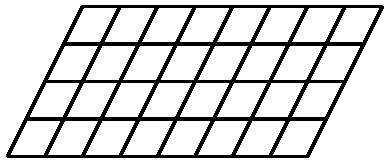
\includegraphics[width=0.55\textwidth]{OKTKH00fig1}
\caption{\label{OKTKH00fig1} %{tilt}
 $\speriod{} \times \period{}$ square lattice with tilt parameter $c$.
 Here, $\speriod{}=8$, $\period{}=4$ and $c=1/4$, so
 $\tilt{}=\speriod{}/4$. The $i$-th site of the first row is identical
 with the mod$(i + c \speriod{},\speriod{})$-th site in the last row. The
 left-most site and the right-most site on the same horizontal line are
 identical.
 }
\end{figure}
%%%%%%%%%%%%%%%%%%%%%%%%%%%%%%%%%%%%%%%%%%%%%%%%%%%%%%%%%%%%%

It is interesting to discuss this problem in terms of the
modular (conformal) transformation.  According to Cardy\rf{Cardy86},
the shape of the 2D lattice may be represented by the imaginary number
\beq
  z = 1/a + i \ c.
\ee{Cardy86-1}
Then, Cardy asserted that the partition function becomes invariant
under the transformations
\beq
  z \rightarrow z + i
\ee{Cardy86-2}
and
\beq
  z \rightarrow 1/z,
\ee{Cardy86-3}
in the limit that the system size becomes infinite.
The first translates, the 2nd inverts: these are easiest to understand in
the complex upper half-plane, see \reffig{ConradSL2Z}.

\item[2021-01-08 Predrag]
Lecian\rf{Lecian13} discusses this group in detail in\\
\arXiv{1303.6343}, see
`big billiard', `small billiard',
Sect.~III.A.  {\em The modular group},
Maass wavefunctions.

%%%%%%%%%%%%%%%%%%%%%%%%%%%%%%%%%%%%%%%%%%%%%%%%%%%%%
\begin{figure}
  \centering
  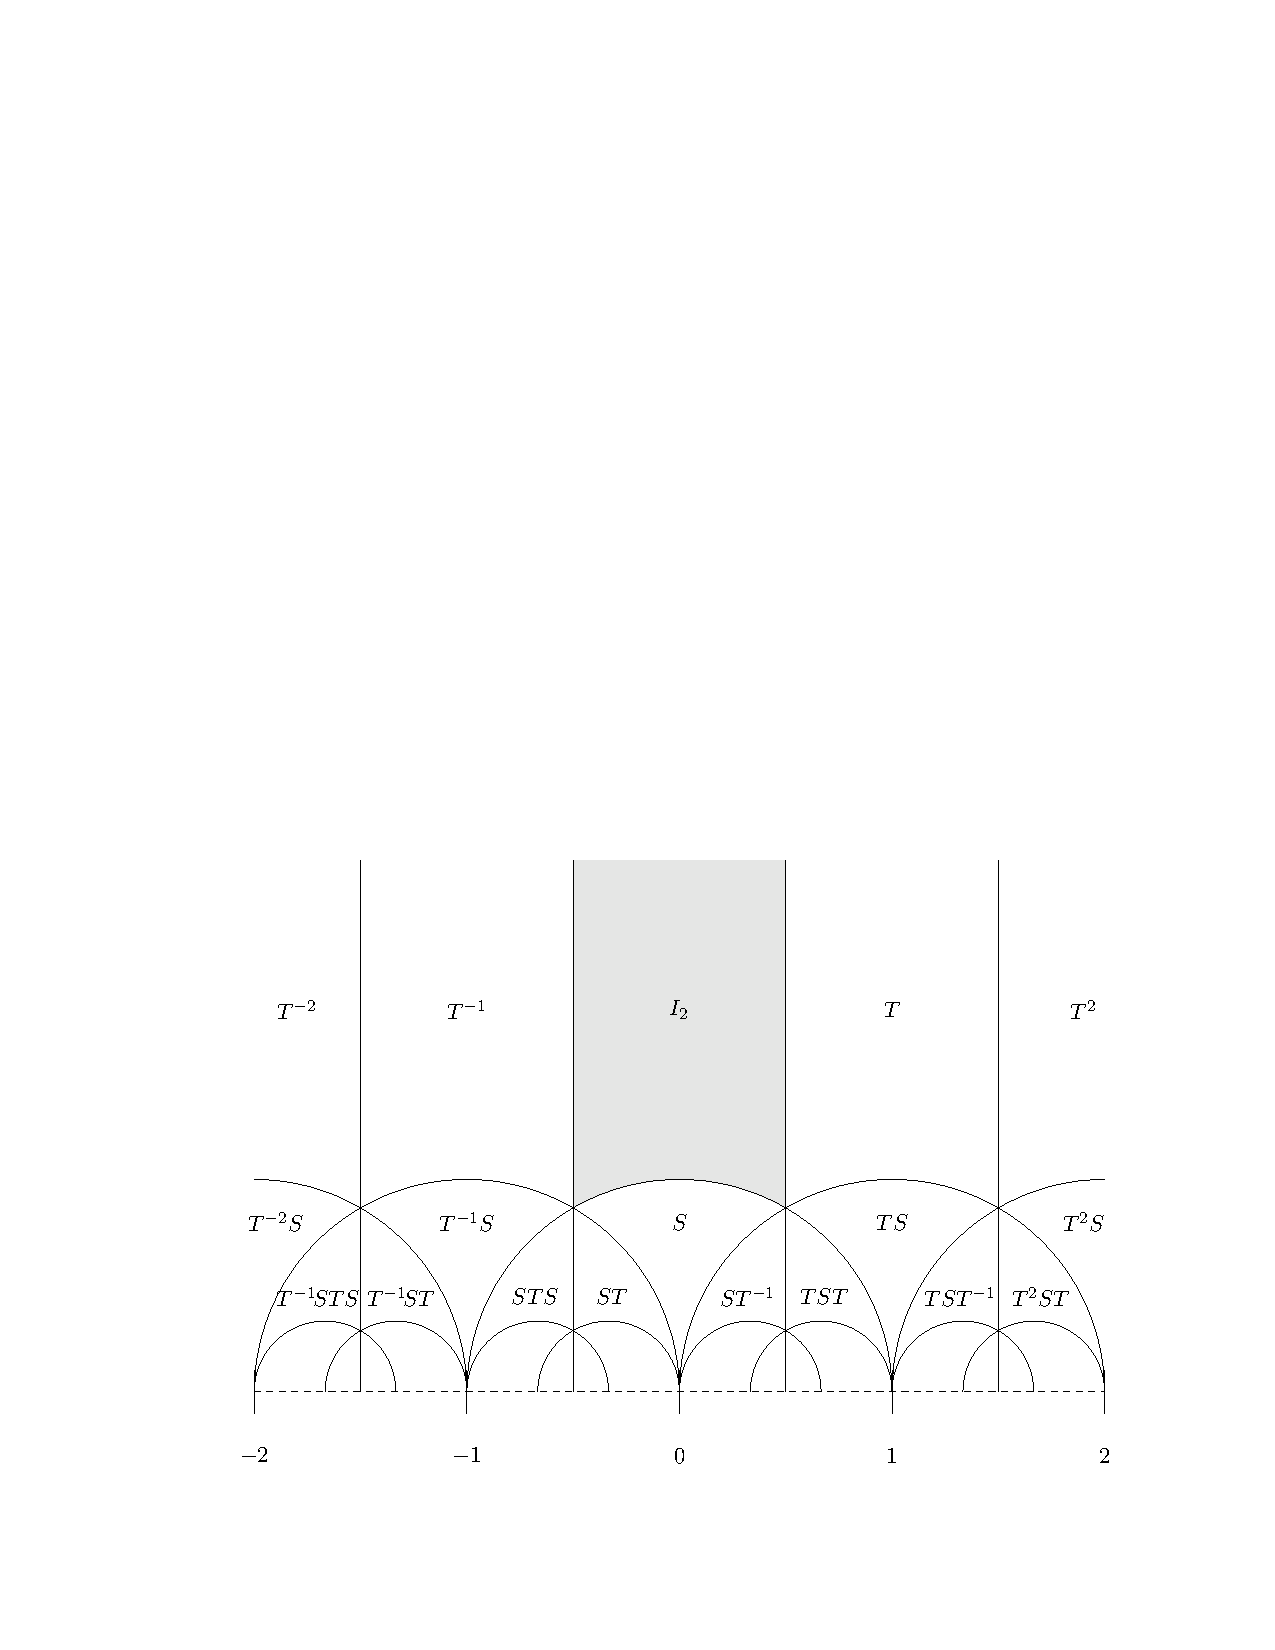
\includegraphics[width=0.74\textwidth]{ConradSL2Z}
  \caption{\label{ConradSL2Z}
Action of \SLn{2}{\integers} on the complex upper half-plane by linear
fractional transformations $T$ and $S$.
Taken from Keith Conrad.
  }
\end{figure}
%%%%%%%%%%%%%%%%%%%%%%%%%%%%%%%%%%%%%%%%%%%%%%%%%%%%%%

We have another invariant transformation
\beq
  z \rightarrow z^*,
\ee{Cardy86-4}
which corresponds to the fact that we can confine $c$ to the interval
of $0 \le c \le 1/2$.
Starting from the recurrence relation
\beq
  z_{n+1} = \frac{1}{z_n+i} + i,
\ee{Cardy86-5}
we can easily show that (recheck! $\period{}$, $\speriod{}$ rewrite wrong
as it stands)
\beq
A=a/(c^2 a^2+1)
 =\frac{\period{}}{\speriod{}}
  \frac{1}{
         \frac{\tilt{}^2}{\speriod{}^2}
         \frac{\period{}^2}{\speriod{}^2}+1
           }
\ee{Cardy86-6}
is an invariant, and can be regarded as the effective aspect ratio.

\item[2020-10-16 Predrag]
For me the problem is that
I do not see any of the above formulas in Cardy\rf{Cardy86},
except for \refeq{Cardy86-1} that might correspond to his
figure of a parallelepiped.
I understand nothing in the paper. He writes thoug
something intriguing:
``the symmetry of the parallelogram, which corresponds to the invariance
of $Z(\delta)$ under the modular group, has recently been exploited to
limit the possible gauge groups in heterotic string theories by
D. Gross, J. Harvey, E. Martinec and R. Rohm, Phys. Rev. Lett. 54 (1985) 502%
%[22]
.'' I would stay far away from such references.


\item[2020-06-19 Predrag]
%\bibitem{zlk99}
Ziff, Lorentz and Kleban\rf{ZiLoKl99}
{\em Shape-dependent universality in percolation},
\arXiv{cond-mat/9811122}.

The torus with a twist has various topological symmetries
that apply to any shape-dependent universal quantity $u(r,t)$.  We consider a rectangular boundary
with base 1 and height $r$, with a horizontal twist $t$ in the
periodic b.~c. \   (Note that having twists in two directions leads to a
non-uniform system, so we don't consider it.) \   $u(r,t)$ satisfies the obvious symmetries
of reflection
\begin{equation}
u(r,t) = u(r,-t)
\label{eq:reflection}
\end{equation}
and  periodicity in the $t$ direction
\begin{equation}
u(r,t) = u(r,1+t)
\label{eq:periodicity}
\end{equation}
Another symmetry follows from the
observation that the same rhombus can be made into a rectangle
in two different ways, leading to:
\begin{equation}
u(r,t) = u\left({r \over r^2 + t^2},{t \over r^2 + t^2}\right)
\label{eq:inverse}
\end{equation}
Another construction
shows that when  $t = 1/n$ where $n$ is an integer,
\begin{equation}
u\left(r,{1 \over n}\right) = u\left({1\over n^2 r},{1 \over n}\right)
\label{eq:integer}
\end{equation}
which also follows from Eqs.\ (\ref{eq:reflection}-\ref{eq:inverse}). On
the complex $\tau = t + ir$ plane, (\ref{eq:inverse}) corresponds to
$\tau \to 1/\tau$ while (\ref{eq:periodicity}) corresponds to $\tau \to
\tau + 1$.  These transformations generate the modular group, and
functions invariant under them are called modular.  Thus, $b(r,t)$ must
necessarily be a modular function.

Besides the excess number, another universal
 quantity on a torus is the cross-configuration probability
$\pi_+(r,t)$, which can be expressed in a quite compact form.
Things veer off to Dedekind eta function and such, and Predrag gives up.


%%%%%%%%%%%%%%%%%%%%%%%%%%%%%%%%%%%%%%%%%%%%%%%%%%%%%%%%%%%%%
% (a), (b) FIG. 1 from Liaw \etal\ \arXiv{cond-mat/0512262}
% (c)   is FIG. 2 from Liaw \etal\ \arXiv{cond-mat/0512262}
\begin{figure}
  \centering
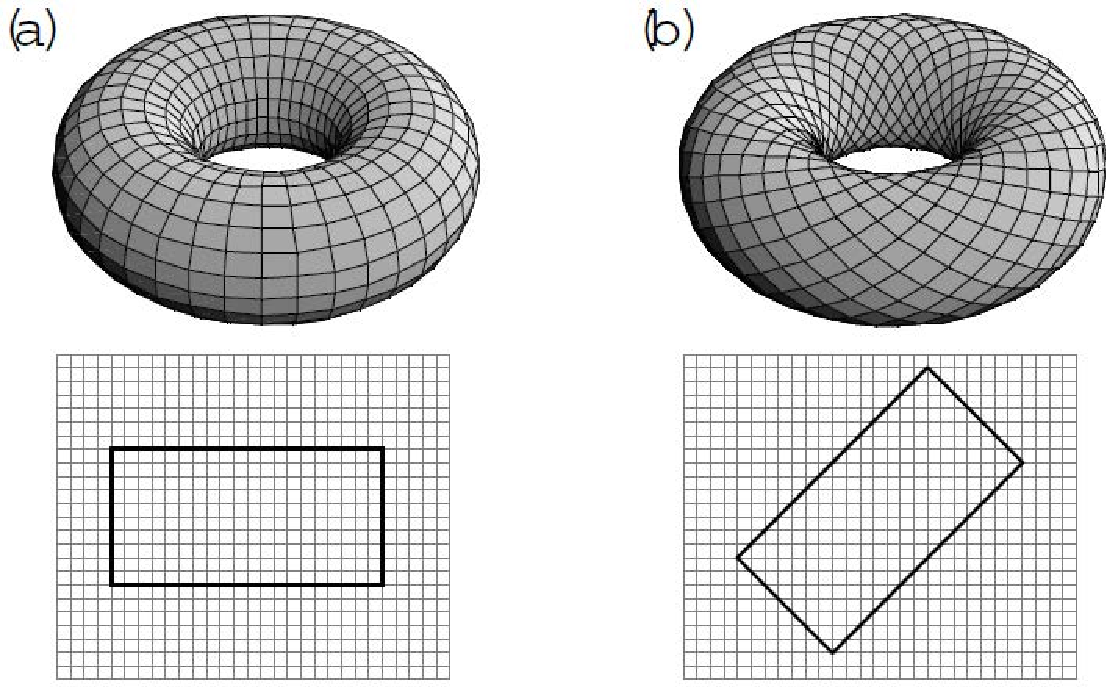
\includegraphics[width=0.55\textwidth]{LHCLL06fig1}
~~~(c) 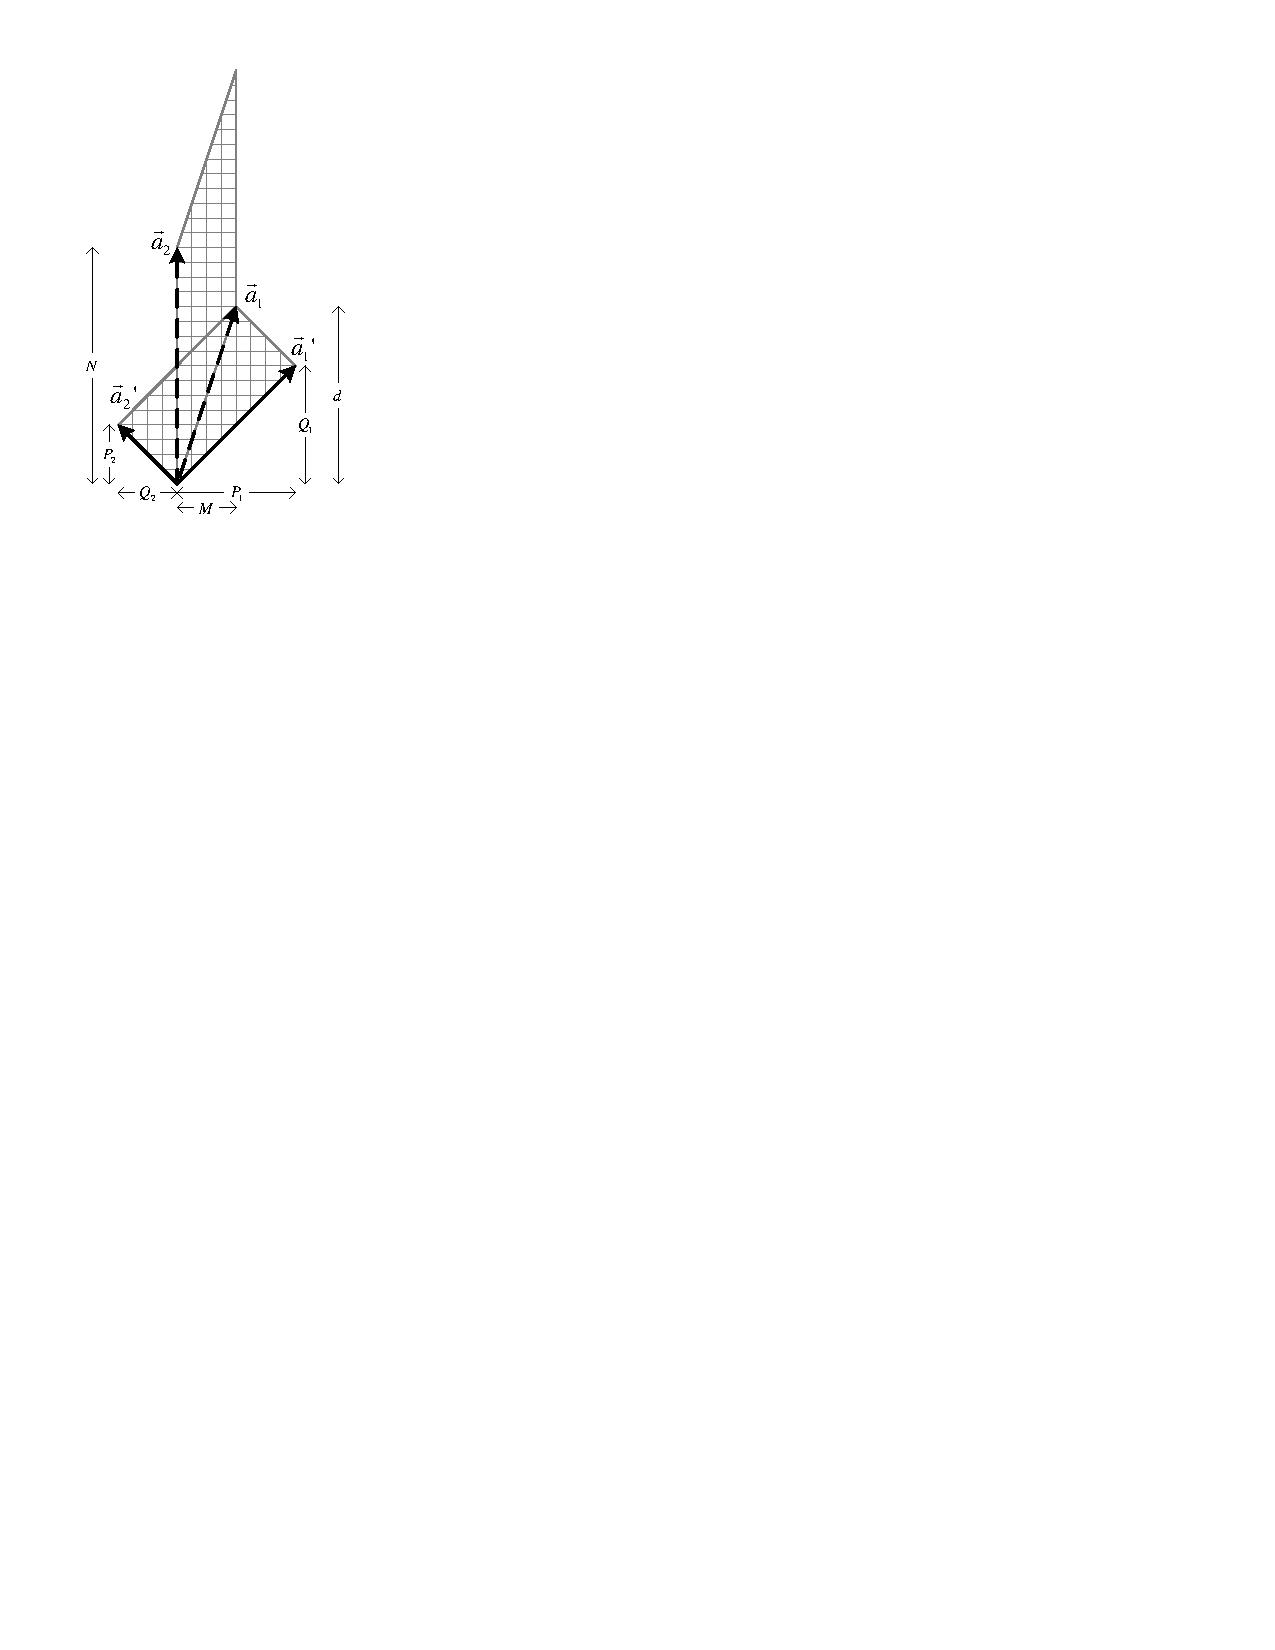
\includegraphics[width=0.25\textwidth]{LHCLL06fig2}
  \caption{\label{LHCLL06fig1}
A helical tiling is formed by pairwise joining of the edges of the
rectangle spanned by an orthogonal set of basis vectors in the
$\integers^2$ lattice:
(a)
    the direction of the basis vectors coincides with the lattice
    orientations for the conventional toroidal \bcs, and
(b)
    a helical torus.
(c)
    Equivalence between the \bcs\ in helical and twisted schemes
    prescribed by $\{{\vec{a}}_{1},{\vec{a}}_{2}\}$ and
    $\{{\vec{a}}_{1}^{\prime},{\vec{a}}_{2}^{\prime }\}$ respectively, on
    a $[M\times N]$ square lattice. For the helical \bcs, the setting
    $Q_{1}/P_{1}=Q_{2}/P_{2}$ ensures that the two primitive vectors are
    orthogonal. On the other hand, twisting is generated by a $d$-unit
    traverse shift.
        }
\end{figure}
%%%%%%%%%%%%%%%%%%%%%%%%%%%%%%%%%%%%%%%%%%%%%%%%%%%%%%%%%%%%%%%

\item[2020-06-19 Predrag]
Liaw \etal\ {\em Exact treatment of Ising model on the helical tori},
\arXiv{cond-mat/0512262}, published as
%
Liaw \etal\rf{LHCLL06} {\em Partition functions and finite-size scalings
of {Ising} model on helical tori}:
The exact closed forms of the partition functions of a two-dimensional
Ising model on square lattices with twisted \bcs\ are given.

A helical
torus is related to the twisted boundary conditions tiling by an
$\SLn{2}{\integers}$ transformation. In $d=2$, the equivalence
transformations among the Bravais cell vector-pairs preserve
the area and are thus $\SLn{2}{\integers}$. This is the prototype of the
modular symmetry of the conformal field theory.%\cite{cardyz}.

In \reffig{LHCLL06fig1} they make a distinction between
the \emph{`helical'}, and the equivalent \emph{`twisted'} tiles.

Helical tori are tiled by pairwise joining the edges of the
rectangle spanned by any orthogonal set of vectors on the lattice plane.
This leads to distinct orientations of the underlying lattice, labelled
by the chirality~{[sahito]} as well as the chiral aspect ratio. The
conventional periodic $BC$ is referred as the helical Bravais cell with trivial
chirality, as depicted in \reffig{LHCLL06fig1}\,(a).

The twisted $BC$  Bravais cell is a modification to the
conventional Bravais cell by cutting the torus and then rejoining after twisting.
Twisted tori are what we call Hermite normal form Bravais cells.
There are two types of twisting: $Tw_{I}(M,N,d/M)$ Bravais cell specified by
 $\{\overrightarrow{a}_{1}=M{\hat{x}}+d{\hat{y}},%
\overrightarrow{a}_{2}=N{\hat{y}}\}$, and $Tw_{II}(M,N,d/N)$ Bravais cell
specified by $\{\overrightarrow{a}_{1}=M{\hat{x}},\overrightarrow{a}_{2}=d{%
\hat{x}}+N{\hat{y}}\}$ used in \refref{CL18}.

In CL18\rf{CL18} notation:
$Tw_{II}(\speriod{},\period{},\tilt{}/\period{})$ Bravais cell is
specified by\\
$\{\overrightarrow{a}_{1}=\speriod{}{\hat{x}},
   \overrightarrow{a}_{2}=\tilt{}{\hat{x}}+\period{}{\hat{y}}\}$.

It suffices to study the
unique correspondence of a helical torus to the one of the above twistings,
say $Tw_{I}$.

The helical tori Bravais cell is given by the orthogonal basis vector pair,
\begin{eqnarray}
{\overrightarrow{a}}_{1}^{\prime } &=&{\hat{x}}\ P_{1}+{\hat{y}}\ Q_{1},
\nonumber \\
{\overrightarrow{a}}_{2}^{\prime } &=&-{\hat{x}}\ Q_{2}+{\hat{y}}\ P_{2},
\label{eq17}
\end{eqnarray}%
where the two radii for the torus are given as
$L_{i}=\sqrt{P_{i}^{2}+Q_{i}^{2}}$ for $i=1,2$. They denoted the helical
system by $Hl(B,L_{1},\chi)$, where the chiral aspect ratio
$B=L_{2}/L_{1}$ and the chirality $\chi =Q_{1}/P_{1}\equiv{Q}_{2}/P_{2}$.
In order to furnish the equivalent structure
$Hl(B,L_{1},\chi)\cong{Tw}_{I}(A,M,\alpha )$,
$\mathcal{M}_{11}={P_{1}}/{M}$ and $\mathcal{M}_{21}=-{Q_{2}}/M$ implies
that
\begin{eqnarray}
\mathcal{M}_{21} &=&-B\chi \mathcal{M}_{11}  \label{eq17_1} \\
1 &=&\mathcal{M}_{11}\mathcal{M}_{22}\ -\ \mathcal{M}_{21}\mathcal{M}_{12}.
\label{eq18} \\
A &=&\frac{\left( \mathcal{M}_{21}\right) ^{2}}{B}+B\left( \mathcal{M}%
_{11}\right) ^{2},  \label{eq19} \\
\alpha &=&-\frac{\mathcal{M}_{21}\mathcal{M}_{22}}{B}-B\mathcal{M}_{11}%
\mathcal{M}_{12}.  \label{eq20}
\end{eqnarray}%

The helical Bravais cell is a subclass of twisted one
by an $\SLn{2}{\integers}$ equivalence relation, \reffig{LHCLL06fig1}\,(c)
and \refeq{eq:inverse}.

They refer to  $\alpha=d/M$  (our notation: $\alpha=\tilt{}/\period{}$)
as a ``twisting factor".

$Q_{M,N}^{\alpha}=Q_{M,N}^{-\alpha }$ as twisting either clockwise or
counterclockwise is not distinguished by the energy. Note that reversing
the sign of a twist factor $\alpha$ is not an $\SLn{2}{\integers}$ transformation.

The $[M\times N]$ square lattice with the helicity factor
$d=D/M$, the system has
periodic boundary conditions in the N direction and
helical (tilted) boundary conditions in the M direction such
that the i-site in the first column is connected with the
$\mod(i+D, M)$th site in the N column of the lattice.

%\bibitem{sahito}
R. Sahito, G. Dresselhaus and M. S. Dresselhaus, \emph{Physical
properties of Carbon Nanotubes}, (Imperial College Press, London, 1998).

%\bibitem{pl} Grassman integral, not relevant here
%V. N. Plechko: Theor. Math. Phys. \textbf{64}, 748 (1985);
%Physica, A \textbf{152}, 51 (1988); Phys. lett. A \textbf{157}, 335 (1991).


Alexi Morin-Duchesne, Paul A. Pearce and Jorgen Rasmussen
{\em Modular invariant partition function of critical dense polymers},
\arXiv{1303.4895}:
% 10.1016/j.nuclphysb.2013.05.016
{[...]} The torus is formed by gluing the top and bottom of the cylinder.
This gives rise to a variety of non-contractible loops winding around the
torus. [...] a parameter v that keeps track of the winding of defects on
the cylinder. [...] The modified trace is constructed as a linear
functional on planar connectivity diagrams in terms of matrix traces
$Tr_d$ (with a fixed number of defects d) and Chebyshev polynomials of
the first kind.

We assume helical boundary conditions in x-direction, i.e.,
\(
\field_{L_x+1,y}=\field_{1,y+1}
\,,
\)
and periodic boundaries in y-direction.

\item[2020-06-16 Predrag]
Izmailian and Hu\rf{IzmHu07}
{\em Finite-size effects for the {Ising} model on helical tori}:
``
We analyze the exact partition function of the Ising model on a square
lattice under helical boundary conditions obtained by Liaw
\etal\rf{LHCLL06}. We find that finite-size corrections for the free
energy, the internal energy, and the specific heat of the model in a
crucial way depend on the helicity factor of the lattice.
''


\item[2019-11-04 Predrag]
\newcommand{\Pf}{\mbox{\rm Pf}\,}
%    \DeclareMathOperator{\Tr}{tr}%
Hobrecht and Hucht\rf{HobHuc18}\\
{\em Anisotropic scaling of the two-dimensional {Ising} model {I:} the torus}:
They compute the partition function and the free energy of the finite
two-dimensional square lattice Ising model with periodic boundary
conditions.

The problem of finding the generating function of the closest-packed
dimer configurations on an arbitrary planar graph was solved by Kasteleyn
in terms of Pfaffians, as it gives the number of \textit{perfect
matchings} of a given directed planar graph with an even number of sites.
This is especially powerful because of the connection between the
Pfaffian and the determinant, namely
\begin{align}
\label{eq:DetPfaffianRel}
	\left(\Pf{\mathcal A}\right)^{2}=\det{\mathcal  A}.
\end{align}
[...]
The nearest-neighbour structure in a row and a column are both
represented by the $[n \times n]$ matrix
%
\begin{align}
	\setlength{\arraycolsep}{8pt}
	{\bf H}_{\mathsf{b},n} = \begin{pmatrix}
		0		& 1	& 0	& \cdots	& 0		\\
		0		& 0 	& 1	&		& 0		\\
		\vdots	&	&	& \ddots	& \vdots	\\
		0		& 0	& 0	&		& 1		\\
		-\mathsf{b}		& 0	& 0	& \cdots	& 0	
	\end{pmatrix},
\end{align}
%
with $\mathsf{b}\in\{+1,0,-1\}$ accounting for
$\mathsf{b}=0$ open, $\mathsf{b}=+1$  periodic, and
$\mathsf{b}=-1$ for anti-periodic boundary conditions.
%, concerning the necessity of transition cycles on the graph to be odd.
$\mathsf{b}=-1$ accounts for periodic boundaries on the
directed graph, i.\,e., in the dimer system, in the sense that all edges
are likewise aligned, while it accounts for antiperiodic BCs in the Ising
model.
However, the topology of the underlying directed graph is not
representative for the Ising model, which is emphasised by the fact that
the Ising partition function is a combination of four Pfaffians.

[...]
the characteristic polynomials are
%
\beq
	\mathcal{P}^{\pm}_{\mathsf{\beta}}(N;\varphi)
    =\prod_{m=0}^{N-1}\left(e^{\pm\ii\varphi}
                        - e^{\ii\varphi_{m}^{(\mathsf{\beta})}}\right)
    = e^{\pm\ii N \varphi} + \mathsf{\beta}
\ee{eq:CharacteristicPolynomialPM}
%
with
%
\begin{align}
	\varphi^{(\mathsf{\beta})}_{m}=\begin{cases}
   		2m\pi/N 		& \text{if } \mathsf{\beta} = -1 \\
   		(2m+1)\pi/N	& \text{if } \mathsf{\beta} = +1
  	\end{cases}
\end{align}
%
for $m\in\{0,1,2,\dots,N{-}1\}$, and thus we will call
$\mathsf{\beta}=-1$ \textit{even} and $\mathsf{\beta}=+1$ \textit{odd}.
Note that the eigenvalues lie equidistantly on the unit circle and thus
we have a free shifting parameter for the spectrum.
We have chosen it in such a way, that the eigenvalue $\varphi_0^{(-)}=0$
appears in the even spectrum; a shift by $-\pi$ on the other hand would
have given rise to a dependency on whether $N$ is even or odd.

Characteristic polynomials \refeq{eq:CharacteristicPolynomialPM} have a
simple scaling form as one only have to replace $\varphi=\Phi/N$ to
obtain
%
\begin{subequations}
\label{eq:CharacteristicPolynomials}
\begin{align}
	\mathcal{P}^{\pm}_{e}(\Phi)=e^{\pm\ii\Phi}-1,\\
	\mathcal{P}^{\pm}_{o}(\Phi)=e^{\pm\ii\Phi}+1
\,.
\end{align}
\end{subequations}
%
%where the $\pm$ accounts for the two possible choices of the eigenvalue
%$\ee^{\pm\ii\varphi^{(\cM)}_{m}}$ in \refeq{eq:HDiagonal}.

They compute variety of determinants. Particularly suggestive is the
product formula for translational invariance in both directions, their
eq.~(2.32), that looks like Han's determinant. This was previously
computed by McCoy \& Wu for the anisotropic torus\rf{McCWu73}.
There is an interesting matrix for the torus, their eq.~(4.3).
All in all, looks harder than what we need for the \catlatt.

\item[2019-11-04 Predrag]

Baxter\rf{Baxter16} {\em The bulk, surface and corner free energies of
the square lattice {Ising} model}

Hucht\rf{Hucht17} {\em The square lattice {Ising} model on the rectangle
{I}: finite systems}

Hobrecht and Hucht\rf{HobHuc20} {\em
Anisotropic scaling of the two-dimensional {Ising} model {II}: surfaces
and boundary fields}

\end{description}

    \newpage
%\section{{Ihara} zeta functions}
%\label{sect:Ihara}
% siminos/spatiotemp/chapter/Ihara.tex
% $Author: predrag $ $Date: 2021-08-10 11:56:19 -0400 (Tue, 10 Aug 2021) $

% called by Ising.tex
\section{{Ihara} zeta functions}
\label{sect:Ihara}

%\newcommand{\Tr}{\mbox{\rm tr}\,}
\renewcommand{\Tr}{\mbox{Tr}\,}

\begin{description}

    \PCpost{2020-05-12}{.
\begin{itemize}
  \item
I think it should be little work to verify for \templatt\ that the Boss
determinant \refeq{gridZeta}, \refeq{Rangarajan2}, \refeq{Rangarajan2a}
for the Ihara zeta function (that counts undirected loops) is the Isola's
Bowen-Ruelle zeta \refeq{Ising:Isola90-13}.
This counts walks of the cat map directed Markov graph.
  \item
Clair's square 2D lattice \refeq{IharaGrid} presumably counts
1D loops (returning walks) on a 2D lattice. So does
Kasteleyn\rf{Kasteleyn63} elliptic integral of the first kind
\refeq{IsingZeta} (see also \refeq{Cserti00(38)}).
  \item
For \catlatt\ we count 2D tori (Bravais lattices); expect a variable
$z_j$ for every translational symmetry direction, not a single $z$ as in
\refeq{IsingZeta}. In Ising models, one counts the 2D configurations - so
how come Ihara functions can do that? Or can they?
  \item
Explain the relation between a discrete torus and the Cayley graph.
For example, given $n\in\naturals^*$, let $G_n$ denote the Cayley graph
$\left({{\integers}/{n\integers},\left\lbrace{\pm1}\right\rbrace}\right)$.
\end{itemize}
    }

\end{description}


\subsection{Heat equation}
\label{sect:heatEq}
    \PC{2020-03-15}{
I like Elaydi\rf{Elaydi05}'s Sect.~3.5.5 {\em The heat equation}
    }
Let $T_{n\zeit}$ be temperature at spatial site $n$ at time $\zeit$. The
heat equation for temperature field $\mathsf{T}=\{T_{n\zeit}\}$ is
\beq
\pde_\zeit \mathsf{T} = D\,\Laplacian_x \mathsf{T}
\,,
\ee{Elaydi05(3.5.22)}
where $D$ is the diffusion constant. Convert this into an integer lattice
difference equation over a finite spacetime domain by the same rescaling
as for \refeq{forwDer}.
Then the heat difference equation for temperature field
$\mathsf{T}=\{T_{n\zeit}\}$ over a finite tile $\LTS{}{}{}$ is
\beq
\pde_\zeit \mathsf{T} = \beta\,\Laplacian_x \mathsf{T}
\,,
\ee{Elaydi05(3.5.22)a}
In the space and time continuum limits, $\beta$ is related to the
diffusion constant by
\[
  \beta = \frac{\Delta\zeit}{(\Delta x)^2}{\diffCon}
        = \frac{\speriod{}^2}{\period{}}{\diffCon}
  \,.
\]


\subsection{Heat kernel}
\label{sect:heatKernel}

\begin{description}

    \PCpost{2020-05-05}{
Jorgenson and Lang\rf{JorLan01} {\em The ubiquitous heat kernel}
    }

    \PCpost{2020-05-13}{
For general regular graphs with a transitive group action,
in particular the discrete tori,  a zeta function
has been defined in an impressive paper by
Chinta, Jorgenson and Karlsson\rf{ChJoKa14} {\em Heat kernels on regular
graphs and generalized {Ihara} zeta function formulas}:
Let q be a positive integer and $G$ be a (q + 1)-regular graph. There is
an associated heat kernel $K_G(t, x_0, x)$ corresponding to the Laplacian
formed by considering the adjacency matrix on $G$. The building blocks of
$K_G$ are I-Bessel functions, and the number
of geodesics from a fixed base point $x_0$ to $x$ of length $m$.

$N^0_m$ denotes the number of closed geodesics of length $m$ in $G$ with
base point $x_0$.

They give a clear introduction into heat kernels on graphs, the origin
of I-Bessel functions, and the relationto the number of paths.
They also deduce the classical Ihara determinantal formula.

There is a second expression for the heat kernel coming from spectral
considerations. Equating the two expressions for the heat kernel, as in
known approaches to the Poisson summation formula or the Selberg trace
formula, one obtains an identity which is a type of theta inversion
formula. To this identity they apply an integral transform,
a Laplace transform with a change of variables, and
obtain the logarithmic derivative of the Ihara zeta function.

For finite graphs, the classical Ihara zeta function is their Ihara zeta
function raised to the power equaling the number of vertices (by fixing
the base point $x_0$, they can work with infinite graphs). They give a
formula, their Theorem 1.3, for $1/zeta$ as an integral over the spectral
measure for the Laplacian.

They also count geodesics paths, not only closed geodesics paths. That
corresponds to computing the Hurwitz zeta function instead of the Riemann
zeta function, they say.

    }

    \PCpost{2020-05-13}{
Chinta, Jorgenson and Karlsson\rf{ChJoKa10}
{\em Zeta functions, heat kernels, and spectral asymptotics on
degenerating families of discrete tori}:

By a discrete torus we mean the Cayley graph associated to a finite
product of finite cycle groups with the generating set given by choosing
a generator for each cyclic factor.

We examine the
spectral theory of the combinatorial Laplacian for sequences of discrete
tori when the orders of the cyclic factors tend to infinity at comparable
rates. First, we show that the sequence of heat kernels corresponding to
the degenerating family converges, after rescaling, to the heat kernel on
an associated real torus.

We then establish an asymptotic expansion, in
the degeneration parameter, of the determinant of the combinatorial
Laplacian. The zeta-regularized determinant of the Laplacian of the
limiting real torus appears as the constant term in this expansion.

By a classical theorem by Kirchhoff, the determinant
of the combinatorial Laplacian of a finite graph divided by the number of
vertices equals the number of spanning trees, called the complexity, of
the graph. As a result, we establish a precise connection between the
complexity of the Cayley graphs of finite abelian groups and heights of
real tori.

It is also known that spectral determinants on discrete tori
can be expressed using trigonometric functions and that spectral
determinants on real tori can be expressed using modular forms on general
linear groups. Another interpretation of our analysis is thus to
establish a link between limiting values of certain products of
trigonometric functions and modular forms. The heat kernel analysis which
we employ uses I-Bessel functions. Our methods extend
to prove the asymptotic behavior of other spectral invariants through
degeneration, such as special values of spectral zeta functions and
Epstein-Hurwitz–type zeta functions.

 For any $d \geq 1$, let $N =
(n_{1}, \cdots, n_{d})$ denote a $d$-tuple of positive
integers, and consider the product
\begin{equation}\label{ddefinition}
D(N) = \prod\limits_{K \neq 0}\left(2d - 2\cos(2\pi k_{1}/n_{1}) -
\cdots - 2\cos(2\pi k_{d}/n_{d})\right);
\end{equation}
where the product is over all $d$-tuples $K = (k_{1}, \cdots,
k_{d})$ of non-negative integers with $k_{j} < n_{j}$, omitting
the zero vector in the product.

One can view $D(N)$ as a determinant of a naturally defined
matrix from graph theory. Quite generally, associated to any
finite graph, there is a discrete Laplacian which acts on the finite
dimensional space of complex valued functions whose domain of
definition is the space of vertices of the graph.
$D(N)$ is equal to the product of the non-zero eigenvalues of the
Laplacian associated to a graph which we call a discrete torus.

The
$d$-dimensional discrete torus is defined as the product space
$$
DT_{N} = \prod\limits_{j=1}^{d} \ell_{j}{\integers} \backslash
{\integers},
$$

See also

Yamasaki\rf{Yamasaki17} {\em An explicit prime geodesic theorem for
discrete tori and the hypergeometric functions}

Anders Karlsson {\em Spectral zeta functions}, \arXiv{1907.01832}
}

   \item[2020-06-04 Predrag]
Evgeny L. Korotyaev
and Jacob  Schach  M{\o}ller\rf{KorMol17},
korotyaev@gmail.com, jacob@math.au.dk,
\arXiv{1701.03605}:
{\em Weighted estimates for the Laplacian on the cubic lattice}:

The starting point for their analysis is a representation of the
summation kernel of the free resolvent (the propagator) in terms of a
product of Bessel functions.

The momentum representation of the discrete Laplacian: one may
diagonalize the discrete Laplacian, using the (unitary) Fourier transform
$\Phi\colon \ell^2({\mathbb Z}^d)\to L^2({\mathbb T}^d)$, where ${\mathbb T}=\R/(2\pi {\mathbb Z})$. It is
defined by
 \[
 (\Phi f)(k)=\widehat f(k)={1\/(2\pi)^{{d\/2}}}\sum_{n\in
 {\mathbb Z}^d} f_ne^{i n\cdot k},\quad \textup{where} \quad
 k=(k_j)_{j=1}^d\in {\mathbb T}^d.
 \]
Here $k\cdot n = \sum_{j=1}^d k_j n_j$ is the scalar product in $\R^d$.
In the resulting momentum representation of the discrete Laplacian
$\Delta$, we write $\widehat \Delta =\Phi \Delta \Phi^*$. The
Laplacian is transformed into a multiplication operator
\[
(\widehat \Delta \widehat f)(k)=\Bigl(\sum_{j=1}^d \cos k_j\Bigr) \widehat f. %=\sum_{j=1}^d
%\rt(-1+2\cos^2 {k_j\/2}\rt).
\]
The operator $e^{it \Delta}, t\in \R$ is unitary  on $L^2({\mathbb T}^d)$ and has  the
kernel $(e^{it \Delta})(n-n')$, where for $n\in{\mathbb Z}^d$:
\[
\begin{aligned}
\label{DiscAsBessel}
(e^{it \Delta})(n) & ={1\/(2\pi)^{d}}\int_{{\mathbb T}^d}
e^{-i n\cdot k+it \sum_{j=1}^d \cos(k_j)}dk\\
& = \prod_{j=1}^d \Bigl(\frac1{2\pi}\int_0^{2\pi}e^{-in_jk+it\cos(k)}dk\Bigr)
= i^{|n|} \prod_{j=1}^d J_{n_j}(t),
\end{aligned}
\]
where $|n| = n_1+\cdots + n_d$.
Here $J_n(z)$ denotes the Bessel function:
\[\label{BesselFunction}
J_n(t)={(-i)^n\/2\pi}\int_0^{2\pi} e^{in k-i t\cos(k)}dk \qquad \forall \
(n,z)\in {\mathbb Z} \times {\mathbb R}.
\]
The rest is all about bounds, we can safely ignore it.


   \item[2020-05-14 Predrag]
J{\'e}r{\'e}my Dubout Jeremy.Dubout@unige.ch
is a smart cookie. I'm very impressed by
Dubout\rf{Dubout19}
{\em Zeta functions of graphs, their symmetries and extended Catalan numbers},
 \arXiv{1909.01659}:

It is natural to form symmetric functions of the eigenvalues of
operators, in finite dimensions one has  the trace and determinant. In
infinite dimensions things become more complicated. For example, the
determinant of the Laplace operator on a  manifold cannot be directly
defined, but the following the heat kernel function can
\begin{align}
\label{Dubout19:1}
\zeta_M(s)=\sum_{n\in\mathbb{N}} \lambda_n^{-s}
  =\frac{1}{\Gamma(s)}\int_0^\infty \!\!\!
   \tr\left(e^{-t \Delta}\right) t^s \frac{dt}{t}
\,,
\end{align}
for $s$ in the half-plane $\left\{s|\Re(s)>0\right\}$.
Since graphs have a natural Laplacian $\Delta$, Dubout considers sums
over the eigenvalues as in \refeq{Dubout19:1}, and introduces the
\emph{spectral zeta function} of a graph $G$ as
$$
\zeta_G(s)=\int_{\sigma(\Delta)} x^{-s}\mu_\Delta^{\delta_v,\delta_v}(dx)
\,,
$$
where $\mu_\Delta^{\delta_v,\delta_v}(dx)$ is a spectral measure of the
Laplacian. $\zeta_G$ provides an analogue of the right hand side of
\refeq{Dubout19:1} for graphs. Dubout introduces a heat function~$H_t$
for infinite graphs\rf{FriKar17} as an analogue of the heat kernel for
manifolds:
$$
\zeta_G(s)=\frac{1}{\Gamma(s)}\int_0^\infty H^G_t t^s\frac{dt}{t}
\,.
$$
This spectral zeta function recovers both previous definitions for finite
graphs, the lattice  $\integers^d$ and the infinite $d$-regular tree.
Dubout extends the $\integers$ functional equation\rf{FriKar17} to
$\integers^2$. For more general $s$ an $d>2$ the existence of such
symmetries remains unknown. The formula acts can interpreted as a
symmetry for Catalan numbers. Dubout is able to describe $\zeta_G$
explicitly for $G=\integers^d$ as well as for products for integers
values.

Contrary to the compact manifold case, the heat kernel of an infinite
graph is not always a trace-class operator. Instead of taking its trace,
Dubout therefore evaluates it on the rooted graph, at some cost.

The resolvant
$$R(z,\Delta)=\frac{1}{z-\Delta}.$$

The heat kernel of $\integers$ is given by
$$
H_t^\integers =\int_0^4 \frac{e^{-tx}}{\pi\sqrt{x(4-x)}} dx=e^{-2t}I_0(2t)
\,,
$$
where $I_0$ a modified Bessel function of first kind, the same as
\refref{KarNeu06} (up to a factor~$2$, coming from their normalization of
the Laplacian). Dubout extends this result to $\integers^d$ with
$$
H_t^{\integers^d}=e^{-2dt}I_0(2t)^d
\,.
$$
The spectral zeta function of $\integers$ is given by
\bea
\zeta_{\integers}(s)
  &=& \int_{0}^{4} x^{-s}\frac{1}{ \pi\sqrt{x(4-x)}}dx
= \frac {1}{\pi}\int_0^1 4^{-s} x^{-s-\frac{1}{2}} (1-x)^{-\frac{1}{2}}dx
 \continue
 &=& \frac{4^{-s}}{\pi}\mathbf{B}\left({\frac{1}{2}-s,\frac{1}{2}}\right)
=\frac{4^{-s}}{\sqrt\pi}
 \frac{\Gamma\left({\frac{1}{2}-s}\right)}{\Gamma\left({1-s}\right)}
\,,
\eea
where $\mathbf{B},\Gamma$ are the beta and gamma functions.

The function $\zeta_\integers$ is meromorphic over
$\complex\setminus\left\lbrace{\frac{1}{2}, \frac{3}{2}, \dots}\right\rbrace$
and satisfies $$\displaystyle  \zeta_\integers(s)={-2s\choose -s}$$
for any $s$.

For a finite transitive graph $G$ with $n$ vertices, the spectral zeta
function $\zeta_G$ can be written in explicit form, similar to the one in
the first part of Equation \ref{Dubout19:1}, and analytically continued
over $\complex$ with the formula
\beq
\zeta_G(s)=\frac{1}{n}\sum_{\lambda\neq 0}\lambda^{-s}
\,,
\ee{Dubout19:211}
where the sum is over the non-zero eigenvalues of $\Delta_G$. The
Lebesgue's decomposition theorem allows us to split the spectral measure
into an absolutely continuous part, a singular continuous part and a pure
point part. The only issue with $\zeta_G$'s analyticity is the presence
of $0$ in the spectrum: A graph $G$ is finite if and only if $0$ belongs
to the pure point part. Dubout then does some serious analysis.

Dubout introduces a \emph{regularized} determinant. If $G$ is finite and
transitive, then
$\det^*(x+\Delta)=\det(x\unit+\Delta)^\frac{1}{|V_G|}.$
In the case of the regularized determinant for $\integers$, Dubout almost
gets the generating function of the Catalan numbers:
\beq
\det^*(x+\Delta_\integers)=\frac{x}{2}+1+\frac{1}{2}\sqrt{x(4+x)}
    =x+2+\sum_{n\geq 1}  C_n \frac{(-1)^n}{x^{n}}
    \,,
\ee{Dubout19:32}
where $C_n=\frac{1}{n+1}{2n \choose n}$ is the $n$-th Catalan number.
\\
{\bf Predrag}: Amusing, but I've also run into Catalan numbers while
counting rooted trees, back in 1976: Cvitanovi\'c\rf{PCar}
{\em Group theory for {Feynman} diagrams in non-{Abelian} gauge theories}

Dubout computes the standard  characteristic polynomial of the Laplacian
of a cyclic graph, by a new, completely analytical way of obtaining the
coefficients. Given $n\in\naturals^*$, let $G_n$ denote the Cayley graph
$\left({{\integers}/{n\integers},\left\lbrace{\pm1}\right\rbrace}\right)$.
Then
\beq
\det (x+\Delta_{G_n})=\sum_{l=0}^{n-1} {2n-l\choose l}\frac{2n}{2n-l}x^{n-l}
\,.
\ee{Dubout19:36}
The coefficients of $\det(x+\Delta_{G_n})$ can  be computed
numerically using the eigenvalues of $\Delta_{G_n}$. Dubout gets the
our usual discrete Fourier product formula
$$
\det(x+\Delta_{G_n}))=
\prod_{k=0}^{n-1} \left({x+4 \sin^2\left({\frac{k \pi}{n}}\right)}\right)
\,,
$$
but he did not find a way to expand this product into a polynomial with
integers coefficients.
\\
{\bf Predrag}: we should alert him to our integer-points counting formulas!

Dubout then relates the {Ihara zeta function $Z_G$}\rf{Terras10} of a
$d$-regular finite graph $G$
\beq
Z_G(u)=
\left({(1-u^2)^{\frac{(d-2)|V_G|}{2}}\det\left({1-(d-\Delta_G)u+(d-1)u^2}\right)}\right)^{-1}.
\ee{Dubout19:322}
to his spectral zeta function.
Given a $d$-regular finite graph $G$ with $n$ vertex, the Ihara zeta
function of $G$ can be computed as
\beq
Z_G(u)= \left({y_u\det^*\left({x_u+\Delta_G}\right)}\right)^{-n}
\,,
\ee{Dubout19:fe}
with
$y_u=u (1-u^2)^{\frac{d}{2}-1}$ and $x_u=(1-\frac{1}{u})(u(d-1)-1)$.

The  appearance of $|V_G|$  in \refeq{Dubout19:fe} as only an
exponent provides good motivation for defining a modified Ihara zeta
function that extends to infinite graphs:

The \textit{regularized Ihara zeta function} of a  (possibly infinite)
d-regular graph $G$ is defined as
\beq
Z^*_G(u)=
{u^{-1}(1-u^2)^{1-\frac{d}{2}}
 \det^*\left({\left(1-\frac{1}{u}\right)(u(d-1)-1)+\Delta_G}\right)}^{-1}
\,.
\ee{Dubout19:24343}
This coincides with the known one for the Cayley graph of a finitely
generated group.

It follows from \refeq{Dubout19:fe} that if $G$ is finite then
$Z^*_G(u)^{|V_G|}=Z_G(u).$ This allows us to extend the functional
equations  to infinite regular graphs.

The regularized determinant of $\integers$ was calculated in
\refeq{Dubout19:32}, and following \refeq{Dubout19:24343} he obtains
the regularized Ihara zeta function of $\integers$:
\beq
    Z_\integers^*(u) = \begin{cases}
              1 & \text{if } 0<|u| < 1,\\
              u^2 & \text{if } |u| > 1.
          \end{cases}
\ee{Dubout19:henduwqed}
Note the functional equation
$$
Z_\integers^*\left({\frac{1}{u}}\right)= \frac{1}{u^2}Z_\integers^*(u)
\,.
$$

That $Z_\integers^*(u)=1$ for $0<u<1$ is a natural result, as the original
definition of the Ihara zeta function is a generating function of
weighted loops, and $\integers$ does not have any, giving us only $1$ as
generating function. The same argument holds for any tree-like
graph.

   \item[2020-05-14 Predrag]
Lenz, Pogorzelski and Schmidt\rf{LePoSc14} {\em The {Ihara} zeta
function for infinite graphs}, \arXiv{1408.3522}, a very lengthy and
ambitious paper, apparently gives yet another definition of
an Ihara zeta function for infinite graphs.
Dubout was unable do
determine how it compares to his \refeq{Dubout19:322}.
I'm not frisky enough to read this paper, after having gone through
Dubout already today...

\end{description}




\subsection{Clair / Clair14}
\label{sect:Clair14}

For the two dimensional integer lattice a zeta function has been defined
and computed in
Clair\rf{Clair14}
{\em The {Ihara} zeta function of the infinite grid}

\HREF{http://math.slu.edu/~clair/}{Bryan Clair} is a great fan of
\HREF{http://math.slu.edu/~clair/preprints/2013-nov-ams-ucr.pdf}
{Ihara zeta functions}.

Shahriar Mokhtari-Sharghi\rf{ClMoSh01,ClMoSh02} have shown that Ihara's
construction can be extended to infinite graphs on which a discrete group
acts isomorphically and with finite quotient. Their works seems to deal with
trees, not lattices, though Clair\rf{Clair14} does discuss infinite square
lattice, see \refeq{ClairGrid}.

The Ihara zeta function may be considered as a modification of the Selberg
zeta function\rf{Bass92}, and was originally written in terms of the variable
$s$, where $z= q^{-s}$.
One of main properties of the Ihara zeta function is the \emph{determinant
formula}, \ie, that its inverse is the determinant of a matrix-valued
polynomial.
A consequence of the determinant formula is that the Ihara zeta function
meromorphically extends to the whole complex plane, and its completions
satisfy a functional equation.

The main formula in all these papers gives a connection between the zeta
function, originally defined as an infinite product, and the Laplacian of the
graph.

Pollicott\rf{Pollicott01} explains in {\em Dynamical zeta functions} Sect.~3.3
what the Laplacian for a undirected graph is, relates it to the adjacency matrix
in a somewhat obvious way, as we are used to on a lattice. He defines Ihara
for undirected graph
\begin{enumerate}
  \item
the graph G has valency $q + 1$ with $q \geq 2$ (i.e., every vertex has $q +
1$ edges attached)
  \item
there is at most one edge between any two vertices
  \item
there are no edges starting and finishing at the same vertex
\end{enumerate}
He outlines a  proof  of  the Bass determinant formula for
the Bowen-Lanford zeta function.

                                                \toCB
\begin{description}
  \item[Loop:] A closed path in $G$, up to cyclic equivalence, without
backtracking.
  \item[Prime:]
 A loop $p$ which is not a power (a repeat) of another loop.
  \item[Back-track:]
A path has a back-tracking if a subsequence of the form $\cdots,x , y , x ,
\cdots$ appears.
\end{description}

The Ihara zeta function of a finite graph $G$
\beq
\zeta(z) = \prod_p \frac{1}{1-z^\cl{p}}
\ee{ClairIhara}
It is instructive to have a look at the octahedral graph in Clair's talk
above. There is no self-crossing condition, so $\zeta(z)$ always has an
infinity of prime cycles, of arbitrary length (as does any {\tzeta}).

As a power series in $z$, the Ihara zeta has non-negative coefficients,
and thus a finite radius of convergence. However, the inverse of the
Ihara zeta is a polynomial.


Ihara considered the special case of regular graphs (those all of whose vertices have the same degree; i.e., the same number of oriented edges coming out of the vertex). A graph is $k$-regular if every vertex has degree $k$.

Terras\rf{Terras10} defines the  $m \times m$ {\em adjacency} matrix as,
\index{adjacency matrix}
\bea
A_{ij} &=& \left\{
             \begin{array}{ll}
 k & \mbox{if a transition $\pS_j$
       $\rightarrow$ $\pS_i$ is possible in $k$ ways} \\
 2\,\ell_j
   & \mbox{if } i=j \\
 0 & \mbox{otherwise}
    \,,
             \end{array}
               \right.
\label{adj_matTerras}
\eea
where $\ell_j$ is the number of loops at vertex $j$. She then assigns to
every of the $e$ unoriented edges a pair of oriented edges. Her graphs
are finite, connected and undirected, without ``backtracks" and ``tails".
It will usually be assumed that they contain no degree 1 vertices (called
``leaves" or ``hair" or ``danglers"). We will also usually assume the
graphs are not cycles or cycles with hair. A cycle graph is obtained by
arranging the vertices in a circle and connecting each vertex to the 2
vertices next to it on the circle. We will allow our graphs to have loops
and multiple edges. For any closed loop, the equivalence class is the set
of all its cyclic permutations. Two loops are equivalent if they differ
only by the starting vertex.

Terras:
We do not consider zeta functions of infinite graphs here. Nor do we
consider directed graphs. Zeta functions for such graphs are discussed,
for example, by Matthew Horton\rf{Horton07}.

There is no unique factorization into primes. The only nonprimes are
powers of primes. We distinguish prime $p$ from $p^{-1}$ which is the
loop traversed in the opposite direction. All graphs have infinity of
primes, with exception of the cycle graph that has only 2 primes
$p,p^{-1}$, traversing the vertices in the opposite directions.

\textbf{Theorem}\rf{Ihara66,Bass92}:
Consider  a finite connected graph $G$  (without degree 1 vertices) with
$m$ vertices, $e$ unoriented (or undirected) edges, $\mbox{deg }m_i$ the
number of (undirected) edges going into vertex $i$. Let $A$ be the
adjacency matrix, $Q$ be the $m \times m$ diagonal matrix with
$Q_{ii} = \mbox{deg }m_i - 1$,
and
$\Delta_z = I -zA + z^2Q$.
The (vertex) adjacency matrix A of $G$ is a $m \times m$ matrix whose i,j
entry is the number of directed edges from vertex i to vertex j. The
matrix $ Q$ is a diagonal matrix whose j-th diagonal entry is 1 less than
the degree of the j-th vertex. If there is a loop at a vertex, it
contributes 2 to the degree.
\beq
1/\zeta(z) = (1 -z^2)^{e-m} \det\Delta_z
\ee{IharaTheo}
(then comes Riemann Hypothesis for the spectrum of a regular graph $G$,
and Ramanujan graphs).

See {\bf 2020-05-11 Bharatram Rangarajan} \refeq{Rangarajan17:templattGenFct}
below for another derivation of the
same.
\\

Next, consider the `grid' zeta function for $G$
the infinite grid, \ie, a square 2D lattice. Let
$\pi = \integers \times \integers$ be a translation acting on $G$.
The zeta function is still
\beq
\zeta(z) = \prod_{[p]} \frac{1}{1-z^\cl{p}}
\ee{ClairGrid}
where $[p]$ is an equivalence class of loops
under translation by $\pi$:
\beq
1/\zeta(z) = (1 -z^4)^2 (1 -z^6)^4(1 -z^8)^{26}
             (1 -z^10)^{152} \cdots
\ee{IharaGrid}
(look at the 8-loops in Clair's talk - there seems to be an extra factor 2
in loop counting. I only see two 6-loops, not four).

On infinite graphs, the adjacency matrix becomes an
$\ell^2 (\integers \times \integers) \to \ell^2 (\integers \times \integers)$
adjacency operator.
For the infinite grid,
\beq
\Delta_z = I -zA + z^3
\ee{GridAdjec}
There is still a determinant formula for the zeta function:
\beq
1/\zeta_\pi(z) = (1 -z^2) \det_\pi\Delta_z
\,.
\ee{gridZeta}
With $\pi = \integers \times \integers$, $\det_\pi$ is an operator determinant:
\beq
\det_\pi\Delta_z = \exp \Tr_\pi \ln \Delta_z
\,,
\ee{gridZetaTr}
where $\Tr_\pi$ is the trace on the group von Neumann algebra ${\cal N}(\pi)$.

The adjacency operator on a square lattice is essentially the 2D Laplacian.
Clair throws in the 2D Ising, then Kasteleyn\rf{Kasteleyn63} and ends up with
\beq
1/\zeta_\pi(z) = (1 -z^2)  (1 +3z^2) \exp \mathbf{I}(k)
\,,
\ee{IsingZeta}
with a simple set of singularities, and $\mathbf{I}(k)$ is related to an
elliptic integral of the first kind \refeq{Cserti00(38)}, expressed in
terms of theta functions (whose squares are modular forms of weight 1).

\subsection{Ihara blog}
\label{sect:IharaBlog}

\begin{description}

    \PCpost{2016-10-03}{
For further discussion, see
\HREF{https://en.wikipedia.org/wiki/Ihara_zeta_function}{Wiki},
and the notes for equation \refeq{gaphLapl}.

Ihara zeta function for undirected graphs satisfies a functional
equation\rf{Terras10}. The formulation of the graph Riemann Hypothesis in
terms of Ihara zeta function is based on the fact that the adjacency
matrix of an undirected regular graph is symmetric. There is no analogue
of Riemann Hypothesis for directed graphs.

A zeta function of a regular graph G associated to a unitary
representation of the fundamental group of G was developed by
Sunada\rf{Sunada89}.
    }

    \PCpost{2016-10-03}{
I cannot, at the moment, tell the difference between
\HREF{https://en.wikipedia.org/wiki/Ihara_zeta_function} {Ihara} and what
I call the {\tzeta} in \HREF{http://chaosbook.org/}
{ChaosBook.org} (section 18.4; the chapter alone is
\HREF{http://chaosbook.org/chapters/count.pdf} {here}). I find Aizenman's
derivation of 2D Onsager solution beautiful - will have to chew on it.
    }

\PCpost{2018-03-22}{
Trying to incorporate dynamics into a generalized, time-reversal
invariant Laplacian by replacing a time forward cat map $A$ by something
like a time reversal invariant combination $A\transp{A}$:

\emph{Incidence matrix} $B$ entries are $b_{ij}=\pm 1$, depending on whether
$v_i$ is a \emph{target} or a \emph{source}.

For literature and further discussion, see
\refsect{sect:Ihara}~{\em {Ihara} zeta functions}.

For the finite \markGraph\ \reffig{fig:PVAdlerWeiss2HL}\,(d)
and \refeq{2rectTransfMatrEq} the incidence matrix is
   \PCedit{
   ({\bf 2018-05-02 Predrag} as they currently stand, the next two equation
   are wrong - they should be $[\ell\times\ell]$ matrices, not
   2\dmn\ ones. Also, the literature discusses only `simple' graphs, \ie,
   graphs without 1-loops)
           }
\beq
    \left[\begin{array}{c}
\phi'_A \\ \phi'_B
    \end{array}\right]
= B\phi= \left[
\begin{array}{cc}
 2  & 1 \\
 -1 & 1 \\
\end{array}
\right]
\left[\begin{array}{c} \phi_A \\ \phi_B \end{array}\right]
\ee{2rectIncidMatrEq}
and
\beq
B\transp{B}=
\left[
\begin{array}{cc}
 2  & 1 \\
 -1 & 1 \\
\end{array}
\right]
\left[
\begin{array}{cc}
 2  & -1 \\
 1 & 1 \\
\end{array}
\right]
=
\left[
\begin{array}{cc}
 5  & -1 \\
 -1 & 2 \\
\end{array}
\right]
\,.
\ee{2rectBtranspB}
Actually, we need something that acts on the whole chain, some
Toeplitz matrix like
\beq
B\transp{B}
``=''
% \frac{1}{a^2}
 -\,
 \begin{bmatrix}  -2    &  1    &        &     &        &    1 \cr
             1    & -2    &   1    &     &        &      \cr
                  &  1    &  -2    &  1  &        &      \cr
                  &       &   1    &     & \ddots &      \cr
                  &       &        &     &        &    1 \cr
             1    &       &        &     &    1   &   -2
         \end{bmatrix}
\,,
\ee{LattLap}
but with 2 fields $[\phi_{A,t},\phi_{B,t}\transp{]}$ at each site $t$.

{\bf Proposition 17.2.} [Godsil and Royle\rf{GodRoy13}]
Given any directed graph G if B is the incidence matrix of G, A is the
adjacency matrix of G, and D is the degree matrix such that
$D_{ii}=d(v_i)$, then
\beq
B\transp{B} = D - A
\,.
\ee{gaphLapl}
The matrix $L=D-A$ is called the (unnormalized) graph Laplacian of
the graph G.
$B\transp{B}$ is independent of the orientation of G and
D-A is symmetric, positive, semidefinite; that is, the eigenvalues of D.

Each row of L sums to zero (because $\transp{B}{\bf1}=0$). Consequently,
the vector $\bf1$ is in the nullspace of L.

The connection between the incidence matrix of a graph and its Laplacian
is the well-known equation $L=\partial \transp{\partial}$.
}

\PCpost{2021-04-14}{
Fan Chung\rf{Chung96}
\HREF{http://www.math.ucsd.edu/~fan/research/revised.html}
{{\em Spectral Graph Theory}} (revised and improved 2006)
 is the ``bible" of spectral graph theory.
Should read chapter {\em Eigenvalues and the Laplacian of a graph}.

See Gabriel Peyr{\'e}
\HREF{https://twitter.com/gabrielpeyre/status/1208265843945156608} {tweet}.

Daniel A. Spielman
\HREF{http://cs-www.cs.yale.edu/homes/spielman/sagt/}
{{\em Spectral and Algebraic Graph Theory}}
deals with the combinatorial, normalized and random walk version of the Laplacian.

What -I think- is important for us is that any graph Laplacian can be written as
\beq
\lattice= S \transp{S}
\,,
\ee{Ching(1.1)}
}
where $S$ is the matrix whose rows are indexed by the vertices and whose
columns are  indexed  by  the  edges.

Let $\unit$ denote the constant  function  which  assumes  the  value  1
on  each  vertex. This  is an eigenfunction of $\lattice$ with eigenvalue
0.

\PCpost{2018-04-05}{
There might be a related undirected network
model, with a graph Laplacian \refeq{gaphLapl}. In that case a Lagrangian
formulation (in terms of graph Laplacians) might be a more powerful formulation
than their Hamiltonian one. ``Arrow of time'' is perhaps encoded by the
orientations of the links in a directed complex network.
}

    \PCpost{2016-10-05}{
Zeta functions of infinite graphs are discussed, for example, by

Bryan Clair
and Shahriar Mokhtari-Sharghi\rf{ClMoSh01},

Rostislav Grigorchuk and
Andrzej Zuk~[?46] (that one is about Cayley trees).

Guido, Isola, and Lapidus\rf{GuIsLa08a}
{\em Ihara's zeta function for periodic graphs and its approximation in
the amenable case}.

Guido, Isola and Lapidus\rf{GuIsLa09}
{\em A trace on fractal graphs and the {Ihara} zeta function}
    }

\item[2020-12-18 Predrag]
Daniele Guido, Tommaso Isola, and Michel Lapidus\rf{GuIsLa08}
{\em Ihara zeta functions for periodic simple graphs}
\arXiv{math/0605753}:
\beq
  Z(G,u)=Z_G(u)=\prod_{[C]}\frac{1}{(1-u^{[C]})^{1/\Group_C}}
\,,
\ee{GuIsLa08Zeta}
The standard lattice graph $\lattice=\integers^{2}$ endowed with the action of the
group $\Group$ which is generated by the rotation by $\frac{\pi}{2}$
around the point $P$ and the translations by elements $(m,n)\in\integers^{2}$
acting as $(m,n)(v_{1},v_{2}):= (v_{1}+2m,v_{2}+2n)$, for
$v=(v_{1},v_{2})\in V\lattice=\integers^{2}$.
\\ \PCedit{Why face-centered point $P$? why $2m$?
In their example, the length $[C]$ in \refeq{GuIsLa08Zeta}
is the number of group elements that map $C$ into itself (the
`stabilizer'), see \reffig{fig:GuIsLa08cycle2}, not what we need.}

%%%%%%%%%%%%%%%%%%%%%%%%%%%%%%%%%%%%%%%%%%%%%%%
%     \begin{figure}
%	 \centering
%	 {GuIsLa08example2}
%	 \caption{A periodic graph $\lattice$ with its quotient $B=\lattice/\Group$}
%	 \label{fig:GuIsLa08example2}
%     \end{figure}
%     \begin{figure}
%	 \centering
%	 {GuIsLa08cycle1}
%	 \caption{A cycle with $|\Group_{C}|=4$}
%	 \label{fig:GuIsLa08cycle1}
%     \end{figure}
\begin{figure}
	 \centering
	 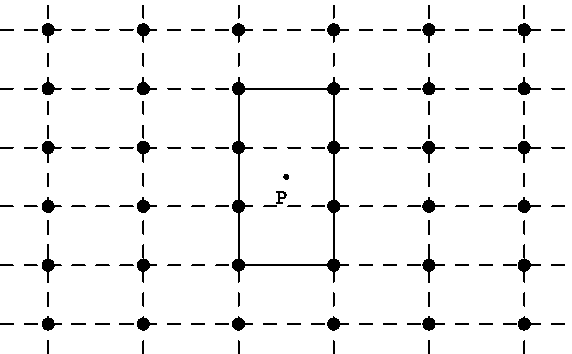
\includegraphics[width=0.5\textwidth]{GuIsLa08cycle2}
	 \caption{A cycle with $|\Group_{C}|=2$}
	 \label{fig:GuIsLa08cycle2}
\end{figure}
%%%%%%%%%%%%%%%%%%%%%%%%%%%%%%%%%%%%%%%%%%%%%%%

The main result in the theory of Ihara zeta functions \refeq{GuIsLa08Zeta}
says that $Z$ is the reciprocal of a holomorphic function, which, up to a
factor, is the determinant of a deformed Laplacian on the graph.


    \PCpost{2016-10-05}{
Unlike in dynamical systems, Ihara zeta functions are defined on
graphs with unoriented (or undirected) edges.

Hashimoto\rf{Hashimoto89}
{\em Zeta functions of finite graphs and representations of p-adic groups}
    }

    \PCpost{2020-05-13}{
Bass\rf{Bass92}
{\em The {Ihara-Selberg} zeta function of a tree lattice}.
It seems that Ihara zeta function walks carry signs - investigate.

He also introduces the \emph{edge zeta function}
to give a determinant form of Ihara zeta function for
undirected graph. This text is from Zhou, Xiao and He\rf{ZhXiHe15},
\arXiv{1502.05771}:

\begin{itemize}
	\item
The \textbf{edge matrix} $W$ of size $[2m \times 2m]$ for an undirected
graph with $m$ undirected edges has entries $w_{ij}$. The $(i,j)$-th
entry of $W$, $w_{ij}$, is a complex variable if the edge $e_i$ is
connected with edge $e_j$ with $e_j \neq e_i^{-1}$, and the entry is 0 if
otherwise.
	\item
For a closed path $C$ in an undirected graph $X$ written as a sequence of
edges $C = e_1e_2 \cdots e_s$, the \textbf{edge norm} of $C$ is
	\[N_E(C) = w_{12}w_{23} \cdots w_{s1}.\]
\end{itemize}
The edge zeta function is defined as follows
\[\zeta_E(W,X) = \prod_{[P] \in \rm{Prime \ Cycles}} (1-N_E(C))^{-1}. \]
It is clear from this definition that if $w_{ij}$ is set to $z \in
\mathbb{C}$, we recover the original Ihara zeta function such that
\[\zeta_G(z) = \zeta_E(W_1,G),\]
where $W_1$ is the edge matrix when all non-zero entries set to $z$.

Furthermore, we have the following formula (cf. Chapter 3 of
Terras\rf{Terras10})
\beq
\zeta_E(W,G) = {\rm Det}(I - W)^{-1}
\,.
\ee{ZhXiHe15:edge_zeta}
    }


    \PCpost{2016-10-05}{
In {\em A Window Into Zeta and Modular Physics}\rf{KirWil10} (that should
warm Li Han's heart) Audrey Terras discusses
\HREF{http://library.msri.org/books/Book57/files/30terras.pdf} {Ihara
zeta function}. She says: ``the Ruelle zeta function of a dynamical
system, will be shown to be a generalization of the Ihara zeta.'' Things
are looking deep. ``It  turns  out  (using  the Ihara  determinant
formula  again)  that  the  Riemann hypothesis means that the graph is
Ramanujan'', etc. She also discusses it in \refref{Terras10} {\em Zeta
Functions of Graphs: A Stroll through the Garden}.

To swoon over the multitude of zetas, read Bartholdi\rf{Bartholdi14} {\em
{Zeta} functions of graphs: a stroll through the garden, by {Audrey
Terras}\rf{Terras10}. Book review}.

Teimoori Faal and M. Loebl\rf{TeiLoe12}
{Bass' identity and a coin arrangements lemma}

Like my \tzeta s,
\HREF{http://kam.mff.cuni.cz/~loebl/clanky/corsica.pdf}{Loebl}'s
Ihara-Selberg function of $G$ is  the infinite product is over the set of
the prime reduced cycles of $G$.

Loebland and Somberg\rf{LoeSom15}
{\em Discrete {Dirac} operators, critical embeddings and {Ihara-Selberg} functions}

da Costa\rf{daCosta16}
{\em The {Feynman} identity for planar graphs}: ``
The Feynman identity (FI) of a planar graph relates the Euler polynomial
of the graph to an infinite product over the equivalence classes of
closed nonperiodic signed cycles in the graph. The main objectives of
this paper are to compute the number of equivalence classes of
nonperiodic cycles of given length and sign in a planar graph and to
interpret the data encoded by the FI in the context of free Lie
superalgebras. This solves in the case of planar graphs a problem first
raised by Sherman and sets the FI as the denominator identity of a free
Lie superalgebra generated from a graph. Other results are obtained
on the zeta functions of graphs.
''

da Costa
{\em Graphs and Generalized Witt identities}
\arXiv{1409.5767}
}

    \PCpost{2016-10-05}{
Sato\rf{Sato05}
{\em Bartholdi zeta functions of group coverings of digraphs}:

The (Ihara) zeta function of a graph G is defined\rf{Ihara66} to be a function of
with u sufficiently small, by
\beq
  Z(G,u)=Z_G(u)=\prod_{[C]}\frac{1}{1-u^{[C]}}
\,,
\ee{Sato05Zeta}
where $[C]$ runs over all equivalence classes
of prime, reduced cycles of G.

 Samuel Cooper and Stratos Prassidis (2010) {\em Zeta functions of infinite
 graph bundles}, % Linear and Multilinear Algebra, 58:2, 185-201,
\HREF{https://doi.org/10.1080/03081080801928084} {DOI} :\\
Originally, Ihara defined the zeta function on finite graphs imitating
the classical definition of the zeta function, where the product is over
all equivalence classes of primitive closed loops C, and $[C]$ denotes
the length of $C$.
    }

    \PCpost{2016-10-05}{
Horton\rf{Horton07}
{\em Ihara zeta functions of digraphs}
considers digraphs whose adjacency matrices are directed edge matrices.

Tarfulea and Perlis\rf{TarPer09}
{An {Ihara} formula for partially directed graphs}: ``
In 2001 Mizuno and Sato showed that the Ihara zeta function of a fully
directed graph has a similar expression, and in 2005, Sato\rf{Sato05} generalized
Ihara's formula to connected, simple, partially directed graphs. (Sato
proved his formula for the more-general two-variable Bartholdi zeta
function.) This paper provides a new proof of Ihara's formula for the
Ihara zeta function of any finite graph, not necessarily connected or
simple, no matter whether it is undirected, fully directed, or partially
directed.
''
    }

    \PCpost{2016-10-30}{
I worry a lot about what time-reversibility means - {\catlatt} is both
time and space reversible, and then there are Ihara zeta functions for
undirected graphs. So I find this interesting: Coppersmith, Kadanoff and
Zhang\rf{CopKadZha01} {\em Reversible {Boolean} networks {I:} distribution of
cycle lengths}. They write: ``
We [...] consider time-reversible dynamics of N Boolean variables models,
with the time evolution of each depending on K of the other variables, which
necessarily have the property that every possible point in the state space is
an element of one and only one cycle. The orbits can be classified by their
behavior under time reversal. The orbits that transform into themselves under
time reversal have properties quite different from those that do not; in
particular, a significant fraction of latter-type orbits have lengths
enormously longer than orbits that are time-reversal symmetric. For large K
and moderate N, the vast majority of points in the state space are on one of
the time-reversal singlet orbits. However, for any finite K, the random
hopping approximation fails qualitatively when N is large enough (N>22K).
When K is large, typical orbit lengths grow exponentially with N, whereas for
small enough K, typical orbit lengths grow much more slowly with N. The
numerical data are consistent with the existence of a phase transition at
which the average orbit length grows as a power of N at a value of K between
1.4 and 1.7. However, in the reversible models, the interplay between the
discrete symmetry and quenched randomness can lead to enormous fluctuations
of orbit lengths and other interesting features that are unique to the
reversible case.
''

Need to check also

Toffoli and Margolus\rf{TofMar90}
{\em Invertible cellular automata: {A} review}

D'Souza and Margolus\rf{SouMar99} {\em Thermodynamically
reversible generalization of diffusion limited aggregation}

}

\item[2020-05-11 Predrag]
Deitmar\rf{Deitmar15} {\em Ihara zeta functions of infinite weighted
graphs}: ``The theory of Ihara zeta functions is extended to infinite
graphs which are weighted and of finite total weight. In this case one
gets meromorphic instead of rational functions and the classical
determinant formulas of Bass and Ihara hold true with Fredholm
determinants.''

\HREF{https://scholar.google.com/citations?hl=en&user=P74k94cAAAAJ}
{Tempesta}\rf{Tempesta15}
{\em A theorem on the existence of trace-form generalized entropies}

Tempesta\rf{Tempesta16} {\em Beyond the {Shannon-Khinchin} formulation:
{The} composability axiom and the universal-group entropy}

\item[2020-05-11 Predrag]
Supriyo Dutta and Partha Guha
{\em Ihara Zeta Entropy},\\
\arXiv{1906.02514};
%Supriyo Dutta and Partha Guha
{\em A System of Billiard and Its Application to Information-Theoretic Entropy},
\arXiv{2004.03444}:
they define Ihara entropy,
an information-theoretic entropy based on the Ihara zeta function of
a graph. A dynamical system consists
of a billiard ball and a set of reflectors correspond to a combinatorial
graph.  The reflectors are represented by the vertices of the graph.
Movement of the billiard ball between two reflectors is represented by the
edges.  The prime cycles of this graph generate the bi-infinite
sequences of the corresponding symbolic dynamical system.  The number
of different prime cycles of a given length can be expressed in terms of
the adjacency matrix of the oriented line graph.  It also constructs the
formal power  series  expansion  of Ihara zeta function.  Therefore,  the
Ihara entropy has a deep connection with the dynamical system of
billiards.

\item[2017-03-08 Predrag]
Reading Band, Harrison and Joyner\rf{BHJ12}
{\em Finite pseudo orbit expansions for spectral quantities of quantum graphs}
one expects to run into another rediscovery of Ihara zeta functions, as the
links are not directed:

``
The \emph{quantum graphs} we consider are metric graphs equipped with a self-adjoint
differential operator $\mathcal{H}$, the Hamiltonian.
Here we are particularly interested in the negative Laplace operator,
\begin{equation}
\mathcal{H}\ :\ f(x)\mapsto-\frac{d^{2}f}{dx^{2}} \ , \label{E:lap_op}
\end{equation}
 or the more general Schr\"odinger operator,
\begin{equation}
\mathcal{H}\ :\ f(x)\mapsto-\frac{d^{2}f}{dx^{2}}+V(x)f(x) \ ,\label{E:schrod}
\end{equation}
 where $V(x)$ is a \emph{potential}, which we assume to be bounded
and piecewise continuous. Note that the value of a function or the
second derivative of a function at a point on the bond is well-defined,
thus it is not important which coordinate, $x_{b}$ or $x_{\hat{b}}$
is used. This is in contrast to the first derivative which changes
sign according to the direction of the chosen coordinate.
''

Indeed, they go through the usual steps of defining oriented graphs and then
putting pairs of oriented bonds on each link, etc. This is explored further
in

Ren, Aleksi{\'{c}}, Emms, Wilson and Hancock\rf{RAEWH10}
{\em Quantum walks, {Ihara} zeta functions and cospectrality in regular graphs}:
review the literature on the discrete-time quantum walks and the Ihara
zeta function.

Setyadi and Stor\rf{SetSto13}
 {\em Enumeration of graphs with the same {Ihara} zeta function}

Higuchi, Konno, Sato and Segawa\rf{HKSS14}
{\em A remark on zeta functions of finite graphs via quantum walks}

Saito\rf{Saito18} {\em A proof of {Terras}' conjecture on the radius of
convergence of the {Ihara} zeta function}
has a nice explicit matrix example, and eigenvalues computation.


    \PCpost{2020-05-05}{
Mizuno and Sato\rf{MizSat01} {\em Zeta functions of digraphs} define a
zeta function of a digraph and an L-function of a symmetric digraph. That
is the usual Bowen-Ruelle (in ChaosBook topological) zeta function.
Tarfulea and Perlis\rf{TarPer09} do note:
``The formula for the zeta function of a directed graph was proved in
1968, wearing a thin disguise, by Bowen and Lanford\rf{BowLan70}. The
elementary connection to directed graphs is made explicit in Th.6.4.6 of
Lind Marcus\rf{LindMar95}.''

Various authors, such as Zhou, Xiao and He\rf{ZhXiHe15} {\em Seiberg
duality, quiver gauge theories, and {Ihara}'s zeta function},
nevertheless refer to it as ``Ihara'', see their Table~2 {\em Ihara zeta
functions for various toric phases of del Pezzo and Hirzebruch quivers}.
Apparently, ``the toric phases are the most popular.''

``The coefficients of the inverse of Ihara zeta function are related to
simple cycles.  In gauge theories, this translates to generic
super-potentials that can be generated from certain quivers.''
This seems to be expansion of a topological zeta function in
terms of fundamental cycles.
    }

    \PCpost{2020-05-05}{
Davey, Hanany and Pasukonis\rf{DaHaPa10}
{\em On the classification of brane tilings}, \arXiv{0909.2868}.
(See also \arXiv{hep-th/0503149}) has an Appendix~A {\em Tiling catalog}.

A brane tiling (or dimer model) is a periodic bipartite graph on the
plane.  Alternatively, we may draw it on the surface of a 2-torus by
taking the smallest repeating structure(known as the fundamental domain)
and identifying opposite edges [1].  The bipartite na-ture of the graph
allows us to colour the nodes either white or black such that white nodes
only connect to black nodes and vice versa.
    }

    \PCpost{2020-05-05}{
Sunada\rf{Sunada13} {\em Topological Crystallography}.
Have the book \CBlibrary{Sunada13}, but do not know how to get useful
info for \catlatt\ out of it.

``the Ihara zeta function [is] a graph-theoretic analogue of class field
theory, discrete Laplacians, and harmonic maps.''

Again, ``Abel–Jacobi maps'' pop up, and again I have no idea what they
are.

    }

    \PCpost{2020-05-06}{
Ren, Wilson and Hancock\rf{ReWiHa11}
{\em Graph characterization via {Ihara} coefficients}:
For an unweighted graph, the Ihara zeta function is the reciprocal of a
quasi characteristic polynomial of the adjacency matrix of the associated
oriented line graph.

First, we demonstrate how to characterize unweighted graphs in a
per\,mut\,ation-invariant manner using the polynomial coefficients from the
Ihara zeta function, i.e., the Ihara coefficients.

Second, we generalize the definition of the Ihara coefficients to
edge-weighted graphs, using the reduced Bartholdi zeta function.

Experimental results reveal that the Ihara coefficients are more
effective than methods based on Laplacian spectra.

Bul{\`{o}}, Hancock, Aziz and Pelillo\rf{BHAP12} {\em Efficient
computation of {Ihara} coefficients using the {Bell} polynomial
recursion}:
They present a method for computing the Ihara coefficients in terms of
complete Bell polynomials and show how the Ihara coefficients can be
efficiently computed provided that the eigenvalues of the adjacency
matrix are known.
}

\item[2020-05-05 Predrag]
Arrigo,
\HREF{https://scholar.google.com/citations?hl=en&user=CKmGEiwAAAAJ}
{Grindrod},  Higham and Noferini\rf{AGHN18}
{\em On the exponential generating function for non-backtracking walks}
do not mention ``Ihara", but seem to derive it anyway from a 3-term recurrence
relation. They write:


We derive an explicit formula for the exponential generating function
associated with non-backtracking walks around both
undirected and directed graphs. Eliminating backtracking
walks in this context does not significantly increase the computational
expense. We show how the new measures may be interpreted in terms of
standard exponential centrality computation on a certain multilayer
network. Insights from this block matrix interpretation also allow us to
characterize centrality measures arising from general matrix functions.

\item[2020-05-11 Predrag]
Bharatram Rangarajan
{\em A combinatorial proof of Bass's determinant formula for the zeta
function of regular graphs}, \arXiv{1706.00851}:
The zeros and poles of the Selberg zeta
function appear in the Selberg trace formula, which relates the
distribution of primes with the spectrum of the Laplace-Beltrami operator
of the surface. The idea of considering closed geodesics as primes
inspired the work of Hashimoto\rf{Hashimoto89}, Bass\rf{Bass92}, Kotani
and Sunada\rf{KotSun00} to come up with an analogous notion in the
discrete setting.

Just like the Selberg zeta function is related to the spectrum of the
Laplace-Beltrami operator of the surface, it is natural to ask if its
discrete analogue, the Ihara zeta function of a graph, is related to the
spectrum of the Laplacian matrix (or the adjacency matrix) of the graph.
Bass\rf{Bass92} gives an expression for the Ihara zeta function of a
graph $G=(V,E)$ as
$$
\zeta_G(t) = \frac{1}{(1-t^2)^{|E|-|V|} \det(I-tA+(D-I)t^2)}
$$
where $A$ is the adjacency matrix of $G$ and $D$ is the diagonal matrix
of degrees of the vertices of $G$, or in other words, $D=diag(A\vec{1})$.
In particular, if $G$ is $d$-regular, then (see \refeq{GridAdjec},
derivation \refeq{Rangarajan2a})
\beq
\zeta_G(t) = \frac{1}{(1-t^2)^{|E|-|V|} \det(I-tA+(d-1)t^2I)}
\ee{Rangarajan2}
gives a way of obtaining the set of poles
of $\zeta_G(t)$.

For a general, partially directed graph see Sato\rf{Sato05} and
Tarfulea and R. Perlis\rf{TarPer09}.

Most proofs Bass's determinant formula start by expressing the zeta
function in terms of not the adjacency matrix $A$ of $G$, but the
adjacency matrix $H$ of the oriented line graph of $G$ (called the
Hashimoto edge-incidence matrix).

In this paper, we shall see a more elementary combinatorial proof of
Bass's determinant formula in the case when $G$ is regular.
The proof goes as
follows:
\begin{itemize}
\item
    The zeta function $\zeta_G({z})$ has an expansion of the form
$$
\zeta_G({z})= \exp\left( \sum \limits_{k=1}^{\infty} N_k \frac{{z}^k}{k} \right)
$$
where for $k \in \integers$, $N_k$ is the number of rooted,
\emph{non-backtracking} cycles in $G$ of length $k$.
\item
    An expression for $N_k$ is not immediate, the starting
    point is the study of non-backtracking walks on $G$. We can construct
    the family $\{A_k\}_{k \in \mathbb{Z}_{\small{\geq 0}}}$ of $n \times
    n$ matrices such that for every $k \in \mathbb{Z}_{\small{\geq0}}$
    and every $v,w \in V$, $(A_k)_{vw}$ is the number of
    non-backtracking walks on $G$ of length $k$ from $v$ to $w$.
\item
    $N_k$ is combinatorially computable from $\Tr(A_k)$.
\item
    $\Tr(A_k)$ is well-understood in terms of the eigenvalues of $A$ and
    a family of Chebyshev polynomials. These ingredients lead to a proof
    of Bass's determinant formula.
\end{itemize}


%\section{Non-backtracking walks and Chebyshev polynomials}
$(A^k)_{vw}$ counts the total number of walks (with backtrackings) on $G$
from $v$ to $w$ of length $k$. Let
$$A_0,A_1,A_2,A_3,\dots$$
be $[n \times n]$ matrices over $\complex$ such that the value $(A_k)_{vw}$
is the number of \emph{non-backtracking} walks on $G$ from $v$ to $w$ of length
$k$. This family $\{A_k\}_{k \in \integers}$ can be recursively defined
using powers of $A$ as follows:
\begin{itemize}
\item $A_0=I$
\item $A_1=A$
\item $A_2=A^2-dI$
\item For $k \geq 3$,
$$A_k=A\,A_{k-1}-(d-1)A_{k-2}$$
\end{itemize}
This recurrence relation shows that the
ordinary (matrix) generating function for the above sequence is
$$\sum \limits_{k=0}^{\infty} {z}^k A_k = (1- {z}^2)I.
  \left( I-{z}A + (d-1){z}^2 I \right)^{-1}$$
\ie, generating function
$$\frac{1-{z}^2}{1-A{z}+(d-1){z}^2}$$

Consider the
family of Chebyshev polynomials of the second kind
$$U_0(x), U_1(x), U_2(x), \dots $$
defined by the recurrence
$$U_0(x)=1$$
$$U_1(x) = 2x$$
and for $k \geq 2$,
$$U_k(x) = U_{k-1}(x)U_1(x) - U_{k-2}(x)$$
and with generating function
$$\sum \limits_{k=0}^{\infty} U_k(x){z}^k = \frac{1}{1-2x{z}+{z}^2}$$

It is easy to see that
$$\sum \limits_{0 \leq j \leq k/2} A_{k-2j} = (d-1)^{k/2} U_k \left( \frac{A}{2\sqrt{d-1}} \right)$$
implying that for $k \geq 2$,
$$A_k = (d-1)^{k/2} U_k \left( \frac{A}{2 \sqrt{d-1}} \right)
      - (d-1)^{k/2-1} U_{k-2} \left( \frac{A}{2 \sqrt{d-1}} \right)$$
This holds for $0 \leq k \leq 2$ as well, if
$$U_m(x) = 0$$
for every $m < 0$. This allows us to work with the above expression for
$A_k$ for \emph{all} non-negative integers $k$.

Taking trace on both
sides,
$$
\Tr(A_k) = (d-1)^{k/2} \sum \limits_{j=0}^{n-1}
             U_k \left( \frac{\mu_i}{2 \sqrt{d-1}} \right)
         -(d-1)^{k/2-1} \sum \limits_{i=0}^{n-1}
             U_{k-2} \left( \frac{\mu_i}{2 \sqrt{d-1}} \right) $$
where
$$d=\mu_0 \geq \mu_1 \geq \dots \geq \mu_{n-1} \geq d$$
are the $n$ eigenvalues of the adjacency matrix $A$. Thus we have an
expression for the trace of $A_k$ as a polynomial in the eigenvalues of
$A$.
% This approach is used in the seminal work of Lubotzky, Phillips and
% Sarnak in their construction of Ramanujan graphs. % \cite{lps},
For a detailed and elementary exposition of Chebyshev polynomials and
non-backtracking walks on regular graphs, the reader is referred to the
monograph by Davidoff, Sarnak and Valette\rf{DaSaVa03}.

While $(A_k)_{vw}$ counts the number of walks on $G$ from vertex $v$ to
vertex $w$ without backtracking, the diagonal element
$(A_k)_{vv}$ does \emph{not} count the number of non-backtracking cycles
of length $k$ rooted at $v$. This is because $(A_k)_{vv}$ also counts
walks of the form
$$e_1 e_2 \dots e_k$$
where $e_{i+1} \neq \overline{e_i}$ for any $1 \leq i \leq k-1$ but
$e_k = \overline{e_1}$. That is, $e_1 e_2 \dots e_k$ is non-backtracking
as a walk from $v$ to $v$, but when considered as a closed walk (or a
loop), the two end edges form a backtracking! Such an instance of a
backtracking that gets overlooked in $\Tr(A_k)$ shall be referred to as a
\emph{tail}.

So $\Tr(A_k)$ counts the number of closed, rooted walks
of length $k$ that could have at most $1$ tail, and hence does \emph{not}
count the  rooted, non-backtracking cycles of length $k$. It is
interesting to ask what the number of closed, rooted non-backtracking
walks of length $k$ is.

Relation between $M_k=\Tr(A_k)$ and $N_k$:
For every $k \geq 3$,
$$N_k = \begin{cases}
M_k - (d-2) (M_{k-2}+M_{k-4}+\dots+M_1) & \text{ odd   }k \\
M_k - (d-2) (M_{k-2}+M_{k-4}+\dots+M_2) & \text{ even }k
\end{cases}$$
By linearity of trace,
$$N_k=\begin{cases}
\Tr\left( A_k - (d-2)(A_{k-2}+A_{k-4}+\dots+A_1) \right) & \text{ if k is odd}\\
\Tr\left( A_k - (d-2)(A_{k-2}+A_{k-4}+\dots+A_2) \right) & \text{ if k is even}\\
\end{cases}$$
[... after a few steps ... this is related to]
$$U_k(x) - U_{k-2}(x) = 2 T_k(x)$$
where $T_k(x)$ is the \emph{Chebyshev polynomial of the first kind}
defined by
\bea
T_0(x) &=& 1\,,\quad
T_1(x)=x
    \continue
T_k(x)  &=&  2x T_{k-1}(x) - T_{k-2}(x)
\quad \mbox{for } k \geq 2
\,,
\label{Rangarajan17:TkRecurr}
\eea
with the generating function
\beq
\sum \limits_{k=0}^{\infty} T_k(x)z^k = \frac{1-xz}{1-2xz+z^2}
\ee{Rangarajan17:TkGenFunct}
[... after a few probably unnecessary steps, ... taking a derivative ...
this is related to]
\begin{align}
N_1{z} + & N_2 \frac{{z}^2}{2} + N_3 \frac{{z}^3}{3} + \dots \\
& = -\frac{n(d-2)}{2} \ln{(1-{z}^2)}
    - \sum \limits_{j=0}^{n-1} \ln{(1-\mu_j {z} + (d-1){z}^2)} \\
& = -\left( \frac{nd}{2} - n \right) \ln{(1-{z}^2)}
    - \ln{\left( \prod \limits_{j=0}^{n-1}1-\mu_j {z} + (d-1){z}^2 \right) }\\
& = -(|E|-|V|) \ln{(1-{z}^2)} - \ln{ \left(\det(I-A{z}+(d-1){z}^2) \right)}
\label{Rangarajan17:templattGenFct}
\end{align}
resulting in \refeq{IharaTheo}:
\\
%\begin{theorem}[Bass's determinant formula]
{\bf Bass's determinant formula}
Let $G=(V,E)$ be a $d$-regular graph with adjacency matrix $A$, and let
$N_k$ count the number of rooted, non-backtracking cycles of length $k$
in $G$. Then
\beq
\zeta_G({z}) = \frac{1}{(1-{z}^2)^{|E|-|V|} \det(I-{z}A+(d-1){z}^2I)}
\ee{Rangarajan2a}
%\end{theorem}









\end{description}

\subsection{Maillard}
\label{sect:Maillard}

Another scary line of literature. Connecting Baxter to dynamical zetas
functions. Maillardinians have a burst at the end of 20th century. Very easy
to collect the literature, as only they cite their own articles, and nobody
else cites them.

A cute cat map exercise - but I have to bike home, will continue
later...

\begin{description}

    \item[2016-11-16 Predrag]
Angl{\`e}s d'Auriac, Boukraa and Maillard\rf{AnBoMa99}
{\em Functional relations in lattice statistical mechanics, enumerative
combinatorics, and discrete dynamical systems} write `` ... non-linear
functional relations appearing in [...] lattice statistical mechanics [...]
We then consider discrete dynamical systems corresponding to birational
transformations. The rational expressions for dynamical zeta functions
obtained for a particular two-dimensional birational mapping, depending on
two parameters [...] compatible with a chaotic dynamical system.

They obsess about the Arnol'd complexity, which counts the number of
intersections between a fixed line  and its $n$th iterate. I do not see why
we should care.

I like Bedford and Diller\rf{BedDil05} {\em Real and complex dynamics of a
family of birational maps of the plane: {The} golden mean subshift} better,
so I follow their notation here. It's a rather impressive paper.

For reasons known to some people (symmetries of Baxter models?) they study a
birational transformation and its inverse,
\bea
\begin{array}{ccl}
 x_{n+1} &=& y_n\,\frac{x_n + a}{x_n - 1}         \\
 y_{n+1} &=& x_n + a - 1
\end{array}
    \qquad
\begin{array}{ccl}
 x_{n-1} &=& y_n + 1-a    \\
 y_{n-1} &=& x_n\,\frac{y_n - aa}{y_n + 1}
\end{array}
\,,\qquad a\in\reals
\,.
\label{eq:AABHM99-3}
\eea
The map is area-preserving in the sense that it preserves a meromorphic
2-form
\[
\frac{dx\wedge dy}{y-x+1}
\]
and is reversible, which means that the map is conjugate to its
inverse via involution $(x,y)\to(-y,-x)$.
The inverse transformation amounts to $y_n\leftrightarrow -z_n$, \ie, the
time reversal symmetry, and the $x-y=0$ line is the \emph{time-reversal
invariant line}.
The {\tzeta} for \refeq{eq:AABHM99-3} is
\beq
\zetatop(z) =  \frac{1 - z - z^2}
                    {1 - z^2}
 \,.
\ee{AABHM99-28}
It counts all \po s, real and complex.
Interestingly, this zeta satisfies an elegant functional relation
relating $\zeta(z)$ and $\zeta(1/z)$.

The zeta function for real roots is complicated and depends on the parameter
$a$.

                                        \toCB
Bedford and Diller\rf{BedDil05} construct a generating partition and the
Markov diagram (they call that Graph of Filtration), including the transient
nodes. The recurrent part of this graph is just the golden mean graph, with
11 repeats forbidden. They obsess much about their ``rectangles.'' Show that
all \po s are hyperbolic. Discuss pre-periodic orbits. Zeta functions are
never mentioned, though topological entropy is computed.

Abarenkova \etal\rf{AABHM99} {\em Rational dynamical zeta functions for
birational transformations} is not worth reading - the material is better
explained in their other papers.

If the dynamical zeta function can be interpreted as the ratio of two
characteristic polynomials of two linear operators  $A$ and $B$, namely
\beq
\frac{1}{\zeta(z)}=\frac{\det(1-zA)}{\det(1-zB)}
\,,
\ee{AABHM99-56a}
then the number of fixed points is given by
\beq
\Tr(A^n)-\Tr(B^n)
\,.
\ee{AABHM99-56b}
In this linear
operators framework, the rationality of the $\zeta$
function\rf{Guckenheimer70,manning}, and therefore the algebraicity of the
exponential of the topological entropy, amounts to having a finite dimensional
representation of the linear operators $A$ and $B$.

Their only explicit example of a rational zeta dynamical
function is the case of the Arnol'd cat map on torus
\(\mathbb{T}^2 =  \reals^2/\integers^2\,,\)
\beq
 {A} =\left(\begin{array}{cc}
 2 & 1 \\
 1 & 1
  \end{array} \right)
\,,\qquad
 {B} =\left(\begin{array}{cc}
 1 & 0 \\
 0 & 1
  \end{array} \right)
\ee{AABHM99-56c}
The {\tzeta}\rf{Isola90} for Arnol'd cat map is
\beq
\zetatop(z)
    = \frac{\det(1-zA)}{\det(1-zB)}
    =  \frac{1 - 3 z + z^2}
                  {(1 - z)^2}
 \,.
\ee{AABHM99-56d}

    \item[2016-06-02, 2020-09-24 Predrag]
From my notes on Isola\rf{Isola90}
{\em {$\zeta$}-functions and distribution of periodic orbits of toral automorphisms},
see \refsect{sect:Isola90}: [...]
The {\tzeta} for cat-map class of models is (see \refeq{AABHM99-46})
\beq
\zetatop(z) % = \frac{(1 - \Lambda z) (1 - \Lambda^{-1} z)}
            %        {(1 - z)^2}
           =  \frac{1 - s z + z^2}
                  {(1 - z)^2}
 \,.
\ee{Ising:Isola90-13}
Define
\beq
d(s)
= {z^{-1} - {s} + z}
\ee{detCat}
then (compare with \refeq{AABHM99-56a})
\beq
  \zetatop(z)
  = \frac{d(s)}{d(2)}
  = 1+\frac{d(s)-d(2)}{d(2)}
  = 1 - {\mu}^2\frac{1}{d(2)}
\ee{zetaCat}

I wonder whether the fact that this is quadratic in $z$ has something to do
with the time-reversibility, and the unsigned graph's Ihara zeta functions?

The ``characteristic function''  \refeq{FGHLW74:charFunct1d}
for the 3-point recurrence centered on the $s$ term, $1/z-s+z$ suggests
multiplying \refeq{Ising:Isola90-13} by $z^{-1}/z^{-1}$. That leads to
\beq
\zetatop(z) = 1 + \frac{{\mu}^2}
                  {(1 - z)(1 -1/z)}
           =  1 + \left(
                   \frac{z}{1 - z} + \frac{1/z}{1 - 1/z}
                  \right){\mu}^2
\,.
\ee{IIsola90-13d}
Interpretation: the \templatt\ zeta function denominator is
the Laplacian, and ${\mu}^2$ is measuring the deviation from the pure Laplacian
case (marginal, no solutions other than the $n=1$ (line of) fixed point(s).

Conversely, given the \tzeta, the generating
function for the number of temporal {\lattstate}s of period $\cl{}$ is
given by the logarithmic derivative of the {\tzeta} \refeq{zetatop-N},
\bea
\sum_{{n}=0}^\infty N_{n} z^{n}
    & = & \frac{2-{s}z}{1 - s z + z^2}-\frac{2}{1 - z}
      =   \frac{2/z-{s}}{1/z - s + z}-\frac{2}{1 - z}
    \continue
& = & \frac{(2/z-{s})(1 - z)-2(1/z - s + z)}{(1/z - s + z)(1 - z)}
    \continue
& = & {\mu}^2\frac{1+z}{(1/z - s + z)(1 - z)}
    \continue
& = & {\mu}^2\left[z + ({s}+2) z^2 + ({s}+1)^2 z^3 \right.
    \ceq
      \left.\qquad\quad
      +\,({s}+2)\,{s}^2 z^4 + (s^2+ s-1)^2 z^5  +  \cdots\right]
\,.
\label{1stChebGenF}
\eea
which is indeed the generating function for $T_{\period{}}(s/2)$, the
Chebyshev polynomial of the first kind.
% of \refeq{POsChebyshev}.

To me it looks like we should include (time reflection symmetry!) also
negative $n$ in the $z^n$ series (Laurent series?), with a negative sign,
so I get
\bea
\sum_{{n}=-\infty}^\infty N_{n} z^{n}
    & = & \frac{{\mu}^2}{z^{-1} - s + z}
    \left(\frac{1+z}{1 - z} {\color{red}-} \frac{1+z^{-1}}{1 - z^{-1}}\right)
    \continue
& = & \frac{{\mu}^2}{z^{-1} - s + z}
    \frac{(1+z)(1 - z^{-1}){\color{red}-}(1 - z)(1 + z^{-1})}{(1 - z)(1 - z^{-1})}
    \continue
& = & \frac{2{\mu}^2}{z^{-1} - {\mu}^2-2 + z}\,\frac{z-z^{-1}}{(1 - z)(1 - z^{-1})}
    \continue
& = & \frac{2{\mu}^2}{z^{-1} - {\mu}^2-2 + z}\,\frac{z^{-1}-z}{z^{-1} - 2 + z}
\,.
\label{1stChebGenFa}
\eea

    \item[2020-09-30 Predrag]
The Bernoulli equation rewritten as a first-order
difference equation:
\beq
\ssp_{\zeit} - {s}\ssp_{\zeit-1} = - \Ssym{\zeit}
\,,\qquad  \ssp_{\zeit} \in [0,1)
\,.
\ee{1stepDiffEq1}
For a Bernoulli system
\bea
\zetatop(z)
 &=&
\exp \left[\ln(1 -  {s}z) - \ln(1 - z) \right]
\continue
 &=&
\frac{1 -  {s}z}{1 - z}
\,.
\label{BernZeta}
\eea
Define
\beq
d(s)
= {z^{-1} - {s}}
\ee{detBernoulli}
then (compare with \refeq{AABHM99-56a})
\beq
  \zetatop(z) = \frac{d(s)}{d(2)}
  = 1+\frac{d(s)-d(2)}{d(2)}
  = 1+ (s-1)\frac{1}{d(2)}
\ee{zetaBernoulli}
The numerator $(1 - {s}z)$ says that a Bernoulli system is a full
shift\rf{CBcount}: there are $s$ fundamental {\lattstate}s and every
other {\lattstate} is built from their concatenations and repeats.

    \item[2020-09-24 Predrag]
For 2\dmn\ \catlatt\ the ``characteristic function''
\refeq{FGHLW74:charFunct1d} the above musings suggests a guess
\bea
\zetatop(z_1,z_2)
&=&
 \frac{z_1 + z_2 - 2{s} + z_1^{-1} + z_2^{-1}}
      {z_1 + z_2 -   4  + z_1^{-1} + z_2^{-1}}
\continue
&=&
1 -
 \frac{2{\mu}^2}
      {z_1 + z_2 -   4  + z_1^{-1} + z_2^{-1}}
\label{PCcatLattZeta1}\\
&=& 1 +
 \frac{2{\mu}^2}
      {(1 - z_1)(1 -1/z_1)+(1 - z_2)(1 -1/z_2)}
\nnu
\eea
If we define
\beq
d(s)
= {z_1 + z_2 - 2{s} + z_1^{-1} + z_2^{-1}}
\ee{detCatLatt}
then (compare with \refeq{AABHM99-56a})
\beq
  \zetatop(z_1,z_2) = \frac{d(s)}{d(2)}
\ee{zetaCatLatt}
suggest some derivatives, integrations with respect to the
parameter ${s}$, resulting in $\ln d(s) - \ln d(2)$ from the
ends of the integration domain.

See also \refeq{AABHM99-56d}.

    \PCpost{2020-05-05}{
Kotani and Sunada\rf{KotSun00} {\em Zeta functions of finite graphs}
seems cited a lot and perhaps belongs to \emph{ChaosBook.org}.
    }

    \PCpost{2020-05-05}{
Stark and Terras\rf{StaTer96}
{\em Zeta functions of finite graphs and coverings}
is cited a lot and perhaps belongs to \emph{ChaosBook.org}.

Stark and Terras\rf{StaTer00}
{\em Zeta functions of finite graphs and coverings, {Part II}}

    }



\end{description}

\renewcommand{\Tr}{\mbox{\rm Tr}\,}
%\newcommand{\Tr}{\mbox{Tr}\,}

%followed by
%\section{$X$-$Y$ model}
%\label{sect:XY}

    \newpage
% siminos/spatiotemp/chapter/models.tex
% $Author: predrag $ $Date: 2021-12-24 01:25:20 -0500 (Fri, 24 Dec 2021) $

\section{Gaussian model}
\label{sect:GaussianModel}
\renewcommand\speriod[1]{{\ensuremath{\ell_{#1}}}}  %continuous spatial period
\renewcommand\period[1]{{\ensuremath{\ell_{#1}}}}  %continuous time period
\renewcommand{\ssp}{\ensuremath{\phi}}             % lattice site field
\renewcommand{\Ssym}[1]{{\ensuremath{m_{#1}}}}    % Boris


\begin{description}
\item[2019-11-04 Predrag]
Ivashkevich, Izmailian and Hu\rf{IvIzHu02} {\em Kronecker's double series
and exact asymptotic expansions for free models of statistical mechanics
on torus}:

{\em Gaussian model} is a boson analog of Ising model. Consider square
lattice of size $N\times M$ wrapped on a torus. To each site
$(m,n)$ of the lattice we assign a continuous variable $\field_{mn}$.
The Hamiltonian of the model is
\begin{equation}
H(\field)=-J\sum_{n=0}^{N-1}\sum_{m=0}^{M-1}
\left(\field_{mn}\,\field_{m+1,n}
      -2\field^2_{mn}
      +\field_{mn}\,\field_{m,n+1}
\right)
\,,
\label{BosonHamiltonian}
\end{equation}
with the partition function
%
$$Z(J)=\int_{\reals^{MN}} e^{-H(\field)}~{\rm d}\sigma(\field)$$
%
If the measure ${\rm d}\sigma(\field)$ in the phase space ${\reals^{MN}}$ is
Gaussian
%
$$ {\rm d}\sigma_{\rm
Gauss}(\field)=\pi^{-MN/2}\prod_{n=0}^{N-1}\prod_{m=0}^{M-1}
e^{-\field^2_{mn}}~ {\rm d}\field_{mn} $$
%
the integration can be done explicitly and the partition function
of the free boson model can be written in terms of the partition
function with twisted boundary conditions % Eq.(\ref{Zab})
\begin{equation}
Z_{\alpha,\beta}(\mu)=\prod_{n=0}^{N-1} 2\left| \textstyle{~\!{\rm
sh}\left[M\omega_\mu\!\left(\frac{\pi(n+\alpha)}{N}\right)+i\pi\beta
\right] }\right| \label{Zab1}
\end{equation}
and
parameterization $J^{-1}=4\,{\rm ch}^2\,\mu$ as
\begin{equation}
Z_{\rm Gauss}(\mu)=\left(\sqrt{2}\;{\rm
ch}\,\mu\right)^{MN}~\Big[\;Z_{0,0}(\mu)\;\Big]^{-1}
\label{ZBoson}
\end{equation}
where
\beq
Z^2_{0,0}(\mu)=
\prod_{n=0}^{N-1}\prod_{m=0}^{M-1}4\left[\textstyle{
\;\sin^2\left(\frac{\pi n }{N}\right)+
\sin^2\left(\frac{\pi m}{M}\right)+2\,{\rm sh}^2\mu
\;}\right]
\,.
\ee{Zab00}
This model exhibit phase transition at the point $\mu_c=0$ where
the partition function is divergent. This is due to the presence
of so-called zero mode, i.e. due to the symmetry transformation
$\field_{mn}\to \field_{mn}+{\rm const}$, which leave the Hamiltonian
(\ref{BosonHamiltonian}) invariant. Correlation functions of
disorder operator in this model have been studied by Sato, Miwa
and Jimbo.
    % \cite{SatoMiwaJimbo}.
    % Sato,~M., Miwa,~T. and Jimbo,~M.: {\it Holonomic Quantum Fields V},
    % Publ. RIMS, Kyoto Univ. {\bf 16}, 531 (1980).

The reason why this model is often considered as boson analog of
the Ising model is that one can choose another measure in the
phase space, which makes this model equivalent to the Ising model
considered above
%\begin{equation}
$$ {\rm d}\sigma_{\rm
Ising}(\field)=2^{-MN}\prod_{n=0}^{N-1}\prod_{m=0}^{M-1}
\big[\,\delta(\field_{mn}-1)+\delta(\field_{mn}+1)\,\big]~ {\rm
d}\field_{mn} $$
%\end{equation}
where $\delta$'s are Dirac $\delta$-functions. With such a
definition the variables $\field_{mn}$ can actually take only two
values: $+1$ or $-1$, so that $\field^2_{mn}=1$. In this case
integration can be replaced by summation over discrete values of
$\field_{mn}=\pm 1$ and the Hamiltonian (\ref{BosonHamiltonian})
coincides with the Hamiltonian of the Ising model
(\ref{IsingHamiltonian}) up to a constant.

\item[2020-06-19 Predrag]

Connect to \refeq{ActionPC}?

Recheck {\bf [2019-09-25 PC]}
Levit and Smilansky?

\item[2020-06-19 Predrag]
P. A. P. Moran\rf{Moran73}
{\em A Gaussian Markovian Process on a Square Lattice}
%  DOI: 10.2307/3212495  https://www.jstor.org/stable/3212495
is a very good paper that does all the right stuff with the Gaussian
``model,'' and ends up with the complete elliptic integral of the first
kind \refeq{Cserti00(38)}.

\item[2020-06-19 Predrag]
% not relevant: https://doi.org/10.1103/PhysRevB.31.5954
% not relevant: http://www.icmp.lviv.ua/journal/zbirnyk.21/011/art11.pdf
% Tom Kennedy \HREF{https://www.math.arizona.edu/~tgk/541/chap4.pdf}
% {\em 4  Random walks}

Eduardo Fradkin\rf{Fradkin13} {\em Field Theories of Condensed Matter Physics},
discusses on p.~336
the quantum partition function of the dimer model which is given by the classical
partition function of a discrete Gaussian model in three Euclidean dimensions on
a cubic lattice. See also p.~332, 345 and 354. Not sure how to connect it to our work.

Shankar\rf{Shankar17} {\em Quantum Field Theory and Condensed Matter}
defines the Gaussian model in Eqs.~(13.2), (6.219);
sect~{\em 11.1 The renormalization group: first pass};

Marino\rf{Marino17} {\em Quantum Field Theory Approach to Condensed
Matter Physics}
(see {\em 5.2 Gaussian Functional Integrals}) does not seem to refer to
the Gaussian model.

Chaikin and Lubensky\rf{ChaLub95} {\em Principles of Condensed Matter Physics}
see {\em 5.3 Gaussian integrals},  {\em 5.8.3 Gaussian model}

\emph{Lattice 89: Proceedings of the 1989 Symposium on Lattice Field Theory}
edited by N. Cabbibo, E. Marinari, G. Parisi

\item[2020-09-06 Predrag]
Kadanoff\rf{Kadanoff00} on Gaussian model:  sect.~{\em 3.4 Lattice Green Function}
and many more.
The ``coefficients matrix'' $C$ in Kadanoff eq.~(3.9) is the inverse
of my `propagator' $\Delta$.

A lattice with one field $\ssp_n$ for each site, then we can define a
particularly simple and important problem by giving the coefficient
matrix
Kadanoff eq.~(3.12)
\beq
C   =
\left(\begin{array}{ccccccc}
 {1}& -{K}& 0 & 0 &\dots &0& -{K}\\
 -{K}&  {1}& -{K}& 0 &\dots &0&0 \\
0 & -{K}&  {1}& -{K}&\dots &0 & 0 \\
\vdots & \vdots &\vdots & \vdots & \ddots &\vdots &\vdots\\
0 & 0 & \dots &\dots &\dots  & {1}& -{K}\\
 -{K}& 0 & \dots &  \dots &\dots& -{K}&  {1}
        \end{array} \right)
\,.
\ee{Kadanoff(3.12)}
The on-site interaction normalizes the Gaussian variables, for $K=0$
one gets the usual multi\dmn\ Gaussian.
$-K$ is the nearest neighbor coupling strength,
related to our case be $-{s}\to1$, off-diagonal $1\to-K$, so
the conversion is $s=-1/K$ (I believe).

Fourier transform of the $d$\dmn\ Green's function Kadanoff eq.~(3.19)
\beq
G(q)   = \frac{1}
         {1 - 2K\sum_{j=1}^d \cos(2\pi k_j/\speriod{j})}
         \,,\qquad
         q_j=
\ee{Kadanoff(3.19)}

Compare with \refeq{Harshaw16a} and our Fourier-transformed field for
$k$th discrete $d$\dmn\ Fourier component on
$\speriod{1},\speriod{2},\cdots,\speriod{d}$ torus,
no tilt,
\beq
\hat{\ssp}_k
= \frac{1}{d{s} - 2\sum_{j=1}^d \cos(2\pi k_j/\speriod{j})}\,\hat{\Ssym{}}_k
\,,
\ee{FourieTrField1}
where
\(
k=(k_1,k_2,\cdots,k_d)\,,
\)
so
\beq
K  = \frac{1}
         {d{s}}
\,,
\ee{Kadanoff-us}

Kadanoff eq.~(4.38) shows that the $d$\dmn\ Gaussian model only makes
sense when $K$ is in the interval $[-1/2d,1/2d]$, \ie, if $|{s}|>2$. If
$|K|$ exceeds this limit (Kadanoff says ``dragons live here''), the
Gaussian integrals diverge at infinite q-values, and the whole problem
stops making sense. When there is any qualitative change in behavior of a
many particle system we say that it undergoes a phase transition. The
Gaussian model does so at the two points $K=\pm1/2d$.

I still have some (conceptual) sign problems, as Kadanoff shows that his
allowed values $K$ correspond to harmonic oscillator states. I would like
that to correspond to $|{s}|<2$. I also need to explain why \catlatt\ has
grammar, while Gaussian model has no restrictions... Still do not
understand why all our {\HillDet}s have an ${\mu}^2$ prefactor. Inconclusive.


\end{description}
\renewcommand\speriod[1]{{\ensuremath{L_{#1}}}}  %continuous spatial period
\renewcommand\period[1]{{\ensuremath{T_{#1}}}}  %continuous time period
\renewcommand{\ssp}{x}
\renewcommand{\Ssym}[1]{{\ensuremath{s_{#1}}}}  % ChaosBook


\section{Tight-binding Hamiltonians}
\label{sect:TightBind}
% moved from siminos/spatiotemp/chapter/QFTlatt.tex 2020-11-01

\begin{description}
  \item[2017-09-11 Predrag]
Economou\rf{Economou06} {\em {Green's Functions in Quantum Physics}}
\CBlibrary{Economou06}
contains a vast amount of useful information.
Lattice shows up in chap.~5 {\em Green's Functions
for tight-binding Hamiltonians}. Extracted text:
\end{description}

``[...] the Green's functions for the so-called tight-binding Hamiltonian
(TBH) are calculated. The TBH is of central importance for solid-state
physics because it is the simplest example of wave propagation in
periodic structures. It is also important for quantum physics in general
because it is rich in physical phenomena (e.g., negative effective mass,
creation of a bound state by a repulsive perturbation) and, at the same
time, simple in its mathematical treatment. Thus one can derive simple,
exact expressions for scattering cross sections and for bound and
resonance levels. The multiple scattering formalism is presented within
the framework of the TBH and applied to questions related to the behavior
of disordered systems (such as amorphous semiconductors).''

He studies the Green's functions associated with a class of periodic
Hamiltonians, i.e., Hamiltonians remaining invariant under a translation
by any vector on a regular $d$\dmn\ lattice.

He also considers the more general case where the lattice can be divided
into two interpenetrating sublattices such that each point of sublattice
1 is surrounded by points belonging to sublattice 2; the Hamiltonian
remains invariant under translation by vectors of sublattice 1 or
sublattice 2.

Periodic Hamiltonians are mathematically equivalent to a system of
coupled 1-d harmonic oscillators and, as a result, they describe (by
direct generalization to 3-d) the ionic motions in a crystalline solid.

In this approach one views the solids as being made up of atoms brought
together from an infinite relative distance. It is then natural (following the
usual practice for molecules) to try to express the unknown electronic wave
functions as linear combinations of atomic orbitals (LCAO).
The simplest version of this approach considers
only one atom per primitive crystal cell, only one atomic orbital per atom,
nearest-neighbor coupling only, and orthonormality of the atomic orbitals.
This oversimplified version of the LCAO is known as the tight-binding
model (TBM); the atomic orbital associated with the atom located at site $\ell$
is symbolized by
\beq
w(r-\ell) = \braket{{r}}{\ell}
\,.
\ee{Economou06(5.4)}
The matrix elements of the Hamiltonian within
this subspace are
\beq
H=\sum_\ell\ket{\ell}\epsilon_\ell\bra{\ell}
  + \sum_{\ell m}\ket{\ell}V_{\ell m}\bra{m}
\,.
\ee{Economou06(5.7)}
The diagonal matrix elements are denoted
by $\epsilon_\ell$ and the off-diagonal matrix elements by
$V_{\ell m}$ ($V_{\ell\ell} = 0$).
The periodicity of the Hamiltonian, i.e., its invariance under translations
by a lattice vector $\ell$, implies that
\beq
\epsilon_\ell=\epsilon_0
\ee{Economou06(5.6a)}
\beq
V_{\ell m}=V_{\ell-m}
\,.
\ee{Economou06(5.6b)}
For the sake of simplicity one assumes that
\beq
   V_{\ell m} = \left\{
     \begin{array}{ll}
         V & \mbox{if\ } \ell,m \mbox{ nearest neighbors}\\
         0 & \mbox{otherwise}
     \end{array}
             \right.
\,.
\ee{Economou06(5.9)}
There is only one quantity, $V$, which, following the usual practice in
the literature, can be taken as negative (for s-like orbitals $V$ is
indeed negative).
\beq
H
  =
\left(\begin{array}{ccccccc}
 \epsilon_0& V & 0 & 0 &\dots &0& V \\
 V &  \epsilon_0& V & 0 &\dots &0&0 \\
0 & V &  \epsilon_0& V &\dots &0 & 0 \\
\vdots & \vdots &\vdots & \vdots & \ddots &\vdots &\vdots\\
0 & 0 & \dots &\dots &\dots  & \epsilon_0& V \\
 V & 0 & \dots &  \dots &\dots& V &  \epsilon_0
        \end{array} \right)
\,.
\ee{Economou06(5.9a)}
A negative $V$, in contrast to a positive $V$,
preserves the well-known property that as the energy of real
eigenfunctions increases so does the number of their sign alternation.

The first term on the rhs of \refeq{Economou06(5.7)} describes a particle
that can be trapped around any particular lattice site $\ell$ with an
eigenenergy $\epsilon_\ell$. The second term allows the particle to hop
from site $\ell$ to site $m$ with a transfer matrix element
$V_{\ell{m}}$. The quantum motion associated with the Hamiltonian
\refeq{Economou06(5.7)} is equivalent to the wave motion of the coupled
pendula, see \reffig{Economou06fig5-1}.
%
\begin{figure}
  \centering
  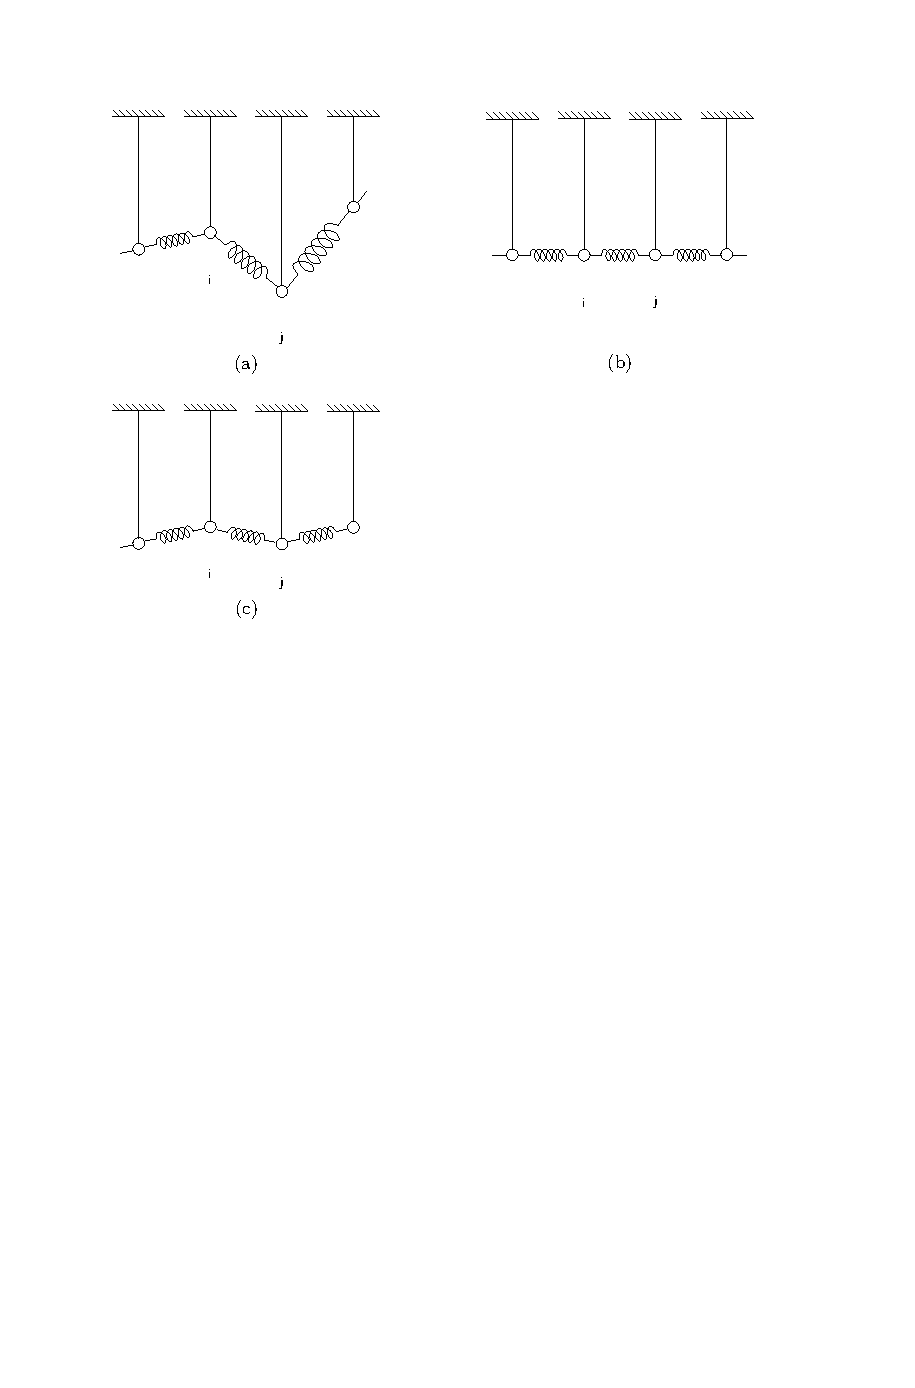
\includegraphics[width=0.70\textwidth]{Economou06fig5-1}
  \caption{
One-dimensional coupled pendulum analog of the tight-binding Hamiltonian,
nearest-neighbor coupling (a). In the periodic case
all pendula and all nearest-neighbor couplings
are identical (b). The double spacing periodic case (c).
(From Economou\rf{Economou06})
  }
  \label{Economou06fig5-1}
\end{figure}
%
\beq
\left(m_i\omega_i^2+\sum_j \kappa_{ij}-m_i\omega^2\right)u_j
- \sum_j \kappa_{ij}u_j=0
\,.
\ee{Economou06(5.13)}
where $u_i$ is the 1-d displacement of the pendulum located at site $i$,
$\omega_i$ is its eigenfrequency in the absence of coupling, and
$\sum_j\kappa_{ij}(u_i-u_j)$ is the force exercised on the pendulum at
the $i$ site as a result of the couplings with all the other pendula;
$m_i$ is the mass at $i$.

If we generalize to 3-d displacements, the problem of coupled pendula is
reduced to that of the ionic (or atomic) motion in solids (by setting
$\omega_i = 0$) since each ion (or atom) is indeed performing small
oscillations around its equilibrium position with the restoring force
being equal to $-\sum_j\kappa_{ij}(u_i-u_j)$. This yields the electronic
eigenfunctions and eigenenergies of the TBM. The eigenmodes are
propagating waves such that the amplitude at each site is the same and
the phase changes in a regular way. For a 2-d square lattice
\beq
E({\bf k}) = \epsilon_0 + 2V[\cos(k_1a)+\cos(k_2a)]
\,,
\ee{Economou06(5.18)}
where $a$ is the lattice constant. In the 1$d$ case, the function
$E({\bf k})$ has an absolute maximum (which corresponds to the upper band
edge) for $k=\pi/a$ or $-\pi/a$ with a value $E_{max}=\epsilon_0+2|V|$;
it has an absolute minimum (which corresponds to a lower band edge) for
$k=0$ with a value $E_{min}=\epsilon_0-2|V|$. Thus the spectrum is a
continuum (a band) extending from $\epsilon_0-2|V|$ to $\epsilon_0+2|V|$.
The bandwidth is $4|V|$.







In his eq.~(5.38) the diagonal
matrix element of the square lattice Greens function is
given by the complete elliptic integral of the first kind\rf{Horiguchi72}
\refeq{Cserti00(38)}.

\bigskip \bigskip

\begin{description}
    \item[2020-10-04 Predrag]
The reason I went above into detail with TBM is (1) it is \catlatt\ for
$s<2$ and (2) has well known elliptic function solutions.
According to
\refeq{Economou06(5.9a)},
the precise formula relating $\epsilon_0$ and $V$ to \catlatt\
stretching factor $s$ is
\[
  s = - \epsilon_0/V
\,,\qquad
u_j \to u_j/\sqrt{-V}
\,.
\]
and the spectrum band extends from $\epsilon_0/|V|-2$ to
$\epsilon_0/|V|+2$, in other words, TBM assumes $|s|<2$.

I assume the band structure for $s<2$ has no counterpart in the hyperbolic,
$s<2$ case, but am not sure.

\PCpost{2018-03-18}{
to Han - can you have a look at the Group Theory course
\HREF{http://birdtracks.eu/courses/PHYS-7143-19/schedule.html\#week8}
{week~8} exercises,
\HREF{http://birdtracks.eu/courses/PHYS-7143-19/soluWeek8Francini.pdf}
{solution~8.3}? I should know this, but I do not, and you have thought
about it: is \catlatt\ in any illuminating sense related to a
tight-binding model? We are not doing QM, but if we formulate the problem
in the continuous space $x\in \reals^d$, rather than the integer lattice
$x\in \integers^d$,  our Hamiltonian is $\delta$ function on each site,
and its neighbors.

If there is a relation, we definitely have to explain that in our paper,
as many colleagues care about couple spin chains and lattices.
}

    \PCpost{2020-01-27}{{\bf to Han -}
For us there is no field $\Xx({z})$ defined over continuum space
$z\in\reals^d$, only $\ssp_z$. Our problems live on the integer lattices
$z\in\integers^d$. This might be called `tight-binding models'. Please
verify whether that's what `tight-binding models' are.
    }

\PCpost{2019-10-10}{Watanabe\rf{Watanabe19}
{\em A proof of the {Bloch} theorem for lattice models}:
``
The Bloch theorem states that the expectation value of the U(1) current
operator averaged over the entire space vanishes for large quantum
systems. The theorem applies as long as all terms in the Hamiltonian are
finite ranged. Finite systems are sensitive to the boundary conditions.
Under the periodic boundary condition, one can only prove that the
current expectation value is inversely proportional to the linear
dimension of the system, while the current expectation value completely
vanishes before taking the thermodynamic limit when the open boundary
condition is imposed. We also provide simple tight-binding models that
clarify the limitation of the theorem in dimensions higher than one.
''
}

    \item[2020-01-13 Predrag]
See also Cserti \etal\rf{Cserti00,CsSzDa11}, in
\refsect{sect:resistors}~{\em Resistor networks}:
The energy-dependent lattice Green's function of the tight-binding
Hamiltonian for a square lattice, his eq.~(30), has energy $E$ playing
the role of our stretching parameter $s$.

\PCpost{2019-07-13}{
Kohler and Cubitt\rf{KohCub19}
{\em Translationally invariant universal classical {Hamiltonians}}
give an explicit construction of a translationally invariant, 2D,
nearest-neighbour, universal classical Hamiltonian with a single free parameter,
drawing on techniques from theoretical computer science, in particular
complexity-theoretic results on tiling problems. Seems too sophisticated for us.
}

  \item[2020-04-19  Predrag]
See also \refchap{chap:chronotope}~{\em Chronotopic literature},
Politi, Torcini and Lepri\rf{PoToLe98}
{\em {Lyapunov} exponents from node-counting arguments}: ``
That resembles the
tight-binding approximation of the lD Schr\"odinger equation (with
imaginary time) in the presence of a random potential, \ie., the Anderson
model.''
\end{description}

\section{Discrete Schr{\"o}dinger equation}
\label{sect:Schrodinger}


\begin{description}
\item[2020-12-06 Predrag]
Marius Lemm, Arka Adhikari and Horng-Tzer Yau, %LeAdYa19
{\em Global eigenvalue distribution of matrices defined by the skew-shift}
\arXiv{1903.11514} study the following question:

\begin{quote}
\emph{Suppose the entries of the large Hermitian matrices $H_N$ are
generated by sampling along the orbits of an ergodic dynamical system. Do
their eigenvalues  still exhibit random matrix statistics, like the
Wigner semicircle law?}
\end{quote}

We will answer this question in the affirmative for the model of $H_N$
defined below, where the underlying dynamical system is generated from
the skew-shift dynamics:
$$
\binom{j}{2} \omega+jy+x \mod 1,
$$
Here $x,y\in \mathbb{T}$ (with $\mathbb{T}$ being the torus) are the
starting positions of the dynamical system and $\omega\in \mathbb{T}$ is
a (typically irrational) parameter called the frequency. The skew-shift
dynamics possesses only weak ergodicity properties, e.g., it is not even
weakly mixing. Nonetheless, it is believed to behave in a quasi-random
way (meaning like an i.i.d.\ sequence of random variables) in various
ways reviewed at the end of the introduction. Moreover, the quasi-random
behavior of the skew-shift should deviate from that of the more rigid
standard shift $j\omega+x\mod 1$ (the circle rotation by an irrational
angle $\omega$). The key difference between the skew-shift and circle
rotation is of course the appearance of a quadratic term $j^2\omega$ for the
skew-shift. This quadratic term has the effect of increasing the
oscillations and thus improving the decay of the exponential sums over
skew-shift orbits. This general fact is a central tenet of analytic
number theory {HL,Mont,W1,W2}, and of our analysis here as well.

{\bf The model.}
Let $\mathbb T$ be the one-dimensional torus, which we identify with
$[0,1]$ in the usual way. For the skew-shift, the role of the ``angle''
is played by the frequency $\omega \in[0,1]$. The skew-shift is then the
transformation
$$
\begin{aligned}
T:&\mathbb{T}^2\to\mathbb{T}^2\\
&(x,y)\mapsto (x+y,y+\omega).
\end{aligned}
$$
We write $T^j$ for the $j$-fold iteration of $T$ and $(T^j(x,y))_1$, for
the first component of the vector $T^j(x,y)\in\mathbb{T}^2$, i.e.,
\beq\label{LeAdYa19:Tjformula}
(T^j(x,y))_1=\binom{j}{2} \omega+jy+x.
\eeq

We consider $2N\times 2N$ Hermitian matrices of the form
$$
H=
\left(\begin{array}{cc} 0&X\\	X^*&0\end{array} \right)
$$
with $X$ an $[N\times N]$ matrix generated from the skew-shift via
\beq\label{LeAdYa19:Xdefn}
X_{i,j}=
\frac{1}{\sqrt{N}}
e\left[\left(\binom{j}{2} \omega_i+jy_i+x_i\right)\right]
\,,\qquad e[t]:=\exp(2\pi i t)
\eeq
Here the $\omega_1,\ldots,\omega_N$ are chosen deterministically (see the
examples below), the $y_1,\ldots,y_N$ in \refeq{LeAdYa19:Xdefn} are sampled
uniformly and independently from $[0,1]$, and the $x_1,\ldots,x_N$ are
arbitrary. (In particular, one can take $x_1=x_2=\ldots=x_N=0$.)

\PCedit{
Predrag: \refeq{LeAdYa19:Xdefn} is an $[N\times N]$ matrix full of
complex phases: it is unlike our 3-banded matrices, I think we can ignore
these papers.
}

Marius Lemm GaTech seminar 2020-04-09: ``
{\em Global eigenvalue distribution of matrices defined by the skew-shift}:
A central question in ergodic theory is whether sequences obtained by
sampling along the orbits of a given dynamical system behave similarly to
sequences of i.i.d. random variables. Here we consider this question from
a spectral-theoretic perspective. Specifically, we study large Hermitian
matrices whose entries are defined by evaluating the exponential function
along orbits of the skew-shift on the 2-torus with irrational frequency.
We prove that their global eigenvalue distribution converges to the
Wigner semicircle law, a hallmark of random matrix statistics, which
evidences the quasi-random nature of the skew-shift dynamics.
''

Kielstra and Lemm  %\rf{KieLem19}
{\em On the finite-size Lyapunov exponent for the Schroedinger operator
with skew-shift potential}
\arXiv{1904.08871}:

A one-dimensional quantum particle living on $\integers$ with energy
$E\in \reals$ is described by the discrete Schr{\"o}dinger equation
\beq\label{LeAdYa19:schr}
\psi_{n+1}+\lambda v_n\psi_n+\psi_{n-1}=E\psi_n,
\eeq
where $\psi=(\psi_n)_{n\in\integers}$ is a sequence in
$\ell^2(\integers;\complex)$. The real-valued potential sequence
$v=(v_n)_{n\in \integers}$ represents the environment that the particle
is subjected to. (The ``coupling constant'' $\lambda>0$ is factored out
for convenience.) Physically, one observes a sudden onset of insulating
behavior in the presence of a random environment (``Anderson
localization''). Mathematically, it is known that for arbitrarily small
$\lambda>0$, the one-dimensional Schr{\"o}dinger operator
\beq\label{LeAdYa19:Hdefn}
(H\psi)_n=\psi_{n+1}+\lambda v_n\psi_n+\psi_{n-1}
\,.
\eeq
has pure point spectrum with exponentially decaying
eigenfunctions\rf{CaKlMa87,KunSou80}.
%\cite{CKM,GMP,KS}.

A natural follow-up question is then: How random does the environment
have to localize the quantum particle? Alternative ``quasi-random''
environments are generated by sampling a nice function along the orbit of
an ergodic dynamical system. This question is interesting from a purely
mathematical ergodic theory perspective, but it also has practical
implications, since computer simulations are mostly based on appropriate
pseudo-random number sequences.

A standing conjecture in this direction concerns the case when the
potential is generated from the nonlinear skew-shift dynamics $T:\mathbb
T^2\to\mathbb T^2$, $T(x,y)=(x+y,y+\omega)$, namely it is of the form
\beq
\label{LeAdYa19:vndefn}
v_n=2\cos\left(\binom{n}{2}\omega +ny+x\right)
\eeq
with $\omega$ irrational (say Diophantine). The key difference between
\refeq{LeAdYa19:vndefn} compared to $v_n=2\cos(n\alpha+\theta)$ is the
appearance of the nonlinear quadratic term $n^2\omega$. The conjecture
states that the associated Schr{\"o}dinger operator $H$ defined by
\refeq{LeAdYa19:Hdefn} is Anderson localized for arbitrarily small
$\lambda>0$ everywhere in the spectrum. Partial results in this vein are
due to
Bourgain %\cite{B}
and
Bourgain-Goldstein-Schlag.  %\cite{BGS}
Note that the conjecture says in particular that the skew-shift dynamics
is appreciably more random-like than the circle rotation where
$v_n=2\cos(n\alpha+\theta)$. (Recall that the latter is only localized
for $\lambda>1$, for us  ${s}>2$.) The observation that the skew-shift is
more quasi-random than the shift has been made in another context by
Rudnick-Sarnak-Zaharescu {RSZ} and others {DR,MY,RS} (concerning the
spacing distribution) and also recently in {ALY} (concerning eigenvalues
of large Hermitian matrices).


\item[2020-12-06 Predrag]
Possibly also of interest:
Marius Lemm and David Sutter
{\em Quantitative lower bounds on the Lyapunov exponent from multivariate
matrix inequalities} \arXiv{2001.09115}:
The Lyapunov exponent characterizes the asymptotic behavior of long
matrix products. Recognizing scenarios where the Lyapunov exponent is
strictly positive is a fundamental challenge that is relevant in many
applications. In this work we establish a novel tool for this task by
deriving a quantitative lower bound on the Lyapunov exponent in terms of
a matrix sum which is efficiently computable in ergodic situations. Our
approach combines two deep results from matrix analysis --- the n-matrix
extension of the Golden-Thompson inequality and the Avalanche-Principle.
We apply these bounds to the Lyapunov exponents of Schrödinger cocycles
with certain ergodic potentials of polymer type and arbitrary correlation
structure. We also derive related quantitative stability results for the
Lyapunov exponent near aligned diagonal matrices and a bound for
almost-commuting matrices.

\item[2020-12-06 Predrag]
Carmona, Klein and Martinelli\rf{CaKlMa87} {\em Anderson localization for
Bernoulli and other singular potentials}:

Bernoulli potentials are potentials that take only two values
\[
\mu  = p\delta(v-a)+ (1-p)\delta(v-b)
\,,\qquad
0<p<1
\,.
\]

Kunz and Souillard\rf{KunSou80} {\em Sur le spectre des op{\'e}rateurs
aux diff{\'e}rences finies al{\'e}atoires} is presumably similar -
models for Anderson localization, we do not need them here.


\end{description}

\section{Harper's model}
\label{sect:Harper}

\begin{description}
\item[2020-12-06 Predrag]
Kielstra and Lemm  %\rf{KieLem19}
{\em On the finite-size Lyapunov exponent for the Schroedinger operator
with skew-shift potential}
\arXiv{1904.08871} write: ``
For example, one can consider
$v_n=2\cos(n\alpha+\theta)$ generated from sampling cosine along an
irrational circle rotation; this is the Harper\rf{Harper55}  or
almost-Mathieu\rf{Simon82} model. It turns out that these linear underlying
dynamics only produce localization for sufficiently strong potentials,
namely only for $\lambda>1$ (for us, ${s}>2$)\rf{Jitomirskaya99}. %{Jit}.
''

%{Jit}
Jitomirskaya\rf{Jitomirskaya99}
{\em Metal-insulator transition for the almost Mathieu operator}.

Svetlana Jitomirskaya, Lyuben Konstantinov and Igor Krasovsky
% \rf{JiKoKr20}
\\
{\em On the spectrum of critical almost Mathieu operators in the rational case}
\\
\arXiv{2007.01005}:

The Harper operator, a.k.a. the discrete magnetic Laplacian
%  name ``discrete magnetic Laplacian'' was first introduced by
%  M. Shubin in \cite{shu}.}, is
a tight-binding model of an electron confined to a 2D square lattice in a
uniform magnetic field orthogonal to the lattice plane and with flux
$2\pi\alpha$ through an elementary cell. It acts on
$\ell^2(\integers^2)$ and
is usually given in the Landau gauge representation
\begin{equation} \label{JiKoKr20(1)} %{alpha}
(H(\alpha)\psi)_{m,n}=\psi_{m,n-1}+\psi_{m,n+1}+e^{-i2\pi\alpha
  n}\psi_{m-1,n}+e^{i2\pi\alpha n}\psi_{m+1,n},
\end{equation}
first considered by Peierls\rf{Peierls33},
who noticed that it makes the
Hamiltonian separable and turns it into the direct integral in $\theta$
of operators on $\ell^2(\mathbb{Z})$ given by:
\begin{equation}
(H_{\alpha, \theta}\,\field)_n  =
   \field_{n-1} + 2\cos2\pi(\alpha n+\theta)\,\field_{n} + \field_{n+1}
\,, \qquad \alpha, \theta \in [0, 1).
\ee{JiKoKr20(2)}
In physics literature, it also appears under the names Harper's or  the
Azbel-Hofstadter model, with both names  used also for the discrete
magnetic Laplacian $H(\alpha)$.  In mathematics, it is universally called
the critical almost Mathieu operator\rf{Simon82}.
% This name was originally introduced by Barry Simon \cite{flu}.
In addition to importance in
physics, this model is of special interest, being at the boundary of two
reasonably well understood regimes: (almost) localization and (almost)
reducibility, and not being amenable to methods of either side.

%{shu}           M.A. Shubin. Discrete Magnetic Laplacian,
%  Commun. Math. Phys. {\bf 164}, 259–275 (1994)

Simon\rf{Simon82}
{\em Almost periodic Schr{\'o}dinger operators: {A review}}\\
{[...]} one-dimensional Schrödinger equation,
$H = -d^2/dx^2 + V(x)$ with $V(x)$
almost periodic and the discrete (= tight binding) analog, i.e., the
doubly infinite Jacobi matrix
\beq
h_{ij} = \delta_{i,j+1}  + V_i\delta_{i,j} + \delta_{i,j-1}
\ee{Simon82}
with $V_n$ almost periodic on the integers.

% {\bf Remark} {\it
% Equations \eqref{Chambersodd} and \eqref{Chamberseven} are variants of
% the well-known Chambers' relation for $H_{\frac{p_0}{q_0}, \theta}$
% \cite{Chambers65} (see \cite{BellissardSimon82} for a proof):

The \emph{Chambers' formula} presents the dependence of the
determinant of the almost Mathieu operator with $\alpha={p}/\cl{}$
restricted to the period $\cl{}$ with Floquet boundary conditions, on
the phase $\theta$ and quasimomentum $k$. In the critical case it is
given by
% (see, e.g., \cite{Last94})
\beq
\det(\jMorb_{\theta, k,\cl{}} - E) =
\Delta(E) -2 (-1)^{\cl{}}(\cos(2 \pi \cl{} \theta) + \cos(k \cl{})),
\ee{JiKoKr20(7)} %{ChambersFormula}
where $\ell \in \mathbb{Z}/\cl{}$, and in our notation
\refeq{JiKoKr20(2)} is written as
\refeq{eq:CatMapNewton5}
\beq
\ssp_{\ell+1}  -  {s}_\ell\, \ssp_{\ell} + \ssp_{\ell-1}
    =
-\Ssym{\ell}
\,,
\ee{Harper}
with site-dependent stretching ${s}_\ell$ (so not a Toeplitz matrix,
compare with \refeq{shiftMatrix}, \refeq{HLdDJacobian},
\refeq{errorVecsTrevers},\refeq{PV2configJ},\refeq{eq:orbitJPVtempJ},
\refeq{catalattLxTrop})
\beq
\jMorb_{\theta, k,\cl{}} :=
\begin{pmatrix}
-{s}_{0} & 1 & 0 & 0 & \cdots & 0 & 0 & e^{-i k \cl{}} \\
1 & -{s}_{1} & 1 & 0 & \cdots & 0 & 0 & 0 \\
0 & 1 & -{s}_{2} & 1 & \cdots & 0 & 0 & 0 \\
\vdots & \vdots & \vdots & \vdots & \ddots & \vdots & \vdots & \vdots \\
0 & 0 & 0 & 0 & \cdots & 1 & -{s}_{\cl{}-2} & 1 \\
e^{i k \cl{}} & 0 & 0 & 0 & \cdots & 0 & 1 & -{s}_{\cl{}-1}
\end{pmatrix}\,,
\ee{JiKoKr20(8)}
compare with the {\jacobianOrb} $\jMorb$ \refeq{jMorbInfin}.
For Harper model, stretching ${s}_\ell$ is given by
\beq
{s}_\ell(\theta) = -2 \cos(2\pi\frac{p}{\cl{}}\ell + \theta)
        \,,\qquad
{s}(x)           = x)
\,,
\ee{JiKoKr20(9)}
and the discriminant $\Delta$
% \footnote{In \cite{Last94}, the discriminant differs from $\Delta(E)$
% by the factor $(-1)^{q_0}$.},
is independent of $\theta$ and $k$.
They obtain a formula of this type for
$\det(B_{\theta, k,\ell} - E).$

\item[2020-12-06 Predrag]
For $\alpha\in\integers$ this is a Helmholtz problem with
stretching parameter ${s}=2\cos 2\pi(\theta)$.

For rational $\alpha$ has periodic ${s}$\rf{Hofstadter76},
as in \refeq{JiKoKr20(9)}.
Note the relative-periodic corner phases $e^{\pm i k q}$
in \refeq{JiKoKr20(8)}).

Hofstadter\rf{Hofstadter76}
{\em Energy levels and wave functions of {Bloch} electrons in rational
and irrational magnetic fields} writes about rational case: ``
Algebra reveals the fact that this condition on $\alpha$ is precisely
that of rationality: We now proceed, making full use of this somewhat
bizarre ansatz.
''

He, as everybody else, sooner or later, rewrites \refeq{Harper} in
the ``\PV\'' `two-configuration representation'\rf{PerViv}
matrix $\jMps$
%=\MatrixII{0}{1}
%          {-1}{s}
\refeq{PerViv:2confRepMat},
\beq
 \left(\begin{array}{c}
 \Delta\field_{\zeit}  \\
 \Delta\field_{\zeit+1}
 \end{array} \right )=
 \left(\begin{array}{cc}
  0 & 1       \\
 -1 & {s}_{\zeit}
 \end{array} \right )
 \left(\begin{array}{c}
 \Delta\field_{\zeit-1}  \\
 \Delta\field_{\zeit}
 \end{array} \right ) %\mbox{ mod } 1
\,.
\ee{CL18:StateSpCatMap}
(note `upside-down' 2D vector), and concerns himself with
the rational,
energy $\tr \jMps^m<2$, oscillatory case.

Note, it's only about the order of recurrence, nobody says the systems
should be Hamiltonian / Lagrangian, works for dissipative systems as
well.

The famed butterfly is a plot
of the eigenvalues for all rational phases $\alpha$.

\item[2020-12-06 Predrag]
        \PCedit{
I am looking at \refeq{JiKoKr20(2)} because this is a different way to
introduce a nonlinearity than the H\'enon CML \refeq{PolTor92(2.1)}
because for irrational $\alpha$
it has a quadratic dependence on the lattice site,
\[
2\cos(2\pi\alpha n) = 2- (2\pi\alpha n)^2 +\cdots
\,.
\]
        }
Nevertheless, this discrete Schr{\"o}dinger is very different from
\templatt, so one more Sunday has been wasted (?) on learning other stuff.

\item[2021-06-25 Indubala Satija]
{\em Geometry, Number Theory and the Butterfly Spectrum of Two-Dimensional
  Bloch Electrons}
\arXiv{2106.1387}:

We take a deeper dive into the geometry and the number theory that underlay
the butterfly graphs of the Harper and the generalized Harper models of Bloch
electrons in a magnetic field. Root of the number theoretical characteristics
of the fractal spectrum is traced to a close relationship between the Farey
tree -- the hierarchical tree that generates all rationals and the Wannier
diagram -- a graph that labels all the gaps of the butterfly graph. The
resulting Farey-Wannier hierarchical lattice of trapezoids provides
geometrical representation of the nested pattern of butterflies in the
butterfly graph. Some features of the energy spectrum such as absence of some
of the Wannier trajectories in the butterfly graph fall outside the number
theoretical framework, can be stated as a simple rule of "minimal violation
of mirror symmetry". In a generalized Harper model, Farey-Wannier
representation prevails as the lattice regroups to form some hexagonal unit
cells creating new {\it species} of butterflies.


\end{description}

\section{Frenkel-Kontorova model}
\label{sect:FrenkelKontorova}

\begin{description}

    \PCpost{2021-02-01}{
The \eqva\ and \reqva\ of Frenkel-Kontorova models\rf{AuAb90}, widely studied in
literature, might be closely related to \henlatt\ and $\phi^4$ lattices.

It is difficult stuff, safely ignored, for now:)

Note the text below
\refeq{MacMei83(17)}
and
\refeq{MraRin12:RR}.

Search for
\textbf{2019-12-12} \emph{Meisinger and Ogilvie} notes in this blog.
    }

\item[2021-02-01 Anna Vainchtein] (U. Pittsburgh)

\emph{Traveling waves in a driven Frenkel-Kontorova lattice}:
Variants of Frenkel-Kontorova model, originally proposed to describe
dislocations in crystal lattices, have been widely used to study a
variety of physical phenomena, including dynamics of twin boundaries and
domain walls, crystal growth, charge-density waves, Josephson junctions
and DNA denaturation. I discuss properties and stability of traveling
waves in chains of Frenkel-Kontorova type driven by a constant external
force. After reviewing some earlier studies for piecewise-smooth variants
of the model, where exact and semi-analytical solutions can be
constructed, I will describe numerical results for a fully nonlinear
damped driven chain from a recent work with J. Cuevas-Maraver (U. of
Sevilla), P.  Kevrekidis (U. of Mass.) and H. Xu (Huazhong U.). In this
setting, \PCedit{traveling wave solutions are computed as fixed points of
a nonlinear map}. [...] Exploring the spectral stability of the obtained
waveforms, we identify, at the level of numerical accuracy of our
computations, a precise criterion for instability of the traveling wave
solutions: monotonically decreasing portions of the kinetic curve always
bear an unstable eigendirection.

The recorded talk will be available
\HREF{https://sites.google.com/view/nwcswebinar/speakers} {here}.
It is a difficult subject, but our case - \eqva\ and \reqva\ is perhaps a
trivial case described in this literature.

\item[2019-06-26 Predrag]
Mramor and Rink\rf{MraRin12}
{\em Ghost circles in lattice {Aubry-Mather} theory}, \arXiv{1111.5963}:

``Monotone lattice recurrence relations such as the Frenkel-Kontorova
lattice, arise in Hamiltonian lattice mechanics as models for
ferromagnetism and as discretization of elliptic PDEs.
They are a multidimensional counterpart of monotone twist maps.''

The paper has an appendix of twist maps, refers to Mather and
Forni\rf{MatFor94} {\em Action minimizing orbits in {Hamiltomian}
systems}. Example of exact symplectic twist maps are the Chirikov
standard map and convex billiards. I think the focus in all this work is
on {\em integrable}, not chaotic:
``Under generic conditions, the Poincar\'e return map of a $2$ degree of
freedom Hamiltonian system near an elliptic equilibrium point is an exact
symplectic twist map. In this case, the corresponding twist map is close
to {\it integrable}, so that it allows for the application of various
kinds of perturbation theory\rf{MatFor94}.''
Lectures on {\em Equidistribution of periodic orbits: An overview of
classical VS quantum results} by Degli Esposti, Graffi, and Isola in {\em
Transition to Chaos in Classical and Quantum Mechanics}\rf{Graffi94} are
also of interest.

Twist maps often admit a variational structure, so that the solutions
$x:\integers^d\to \reals$ are the stationary points of a formal action
function $W(x)$. Given any rotation vector $\omega\in \reals^d$,
Aubry-Mather theory establishes the existence of a large collection of
solutions of $\nabla W(x)=0$ of rotation vector $\omega$. For irrational
$\omega$, this is the {\em Aubry-Mather set}. It consists of global
minimizers and it may have gaps.

The part relevant to our \catlatt\ is the idea of studying globally
stationary solutions by means of a formal gradient. We do not really know
how to find all \twots\ in 2 or more dimensions, even though we know how
to count them, right?
They study the parabolic gradient flow
$\frac{dx}{dt} = -\nabla W(x)$
and prove that every Aubry-Mather set can be
interpolated by a continuous gradient-flow invariant family, the
so-called `ghost circle'. The existence of these ghost circles is known
in dimension $d=1$, for rational rotation vectors and Morse action
functions.

\medskip
{\bf $d$-dimensional Frenkel-Kontorova lattice:}
Here, the goal is to find a
$d$-dimensional ``lattice configuration'' $x:\integers^d\to \reals$ that satisfies
\begin{align}\label{MraRin12:RR}
V'(x_i) - (\Delta x)_i = 0 \  \ \mbox{for all} \ i\in \mathbb{Z}^d
\,.
\end{align}
The smooth function $V: \mathbb{R} \to \mathbb{R}$
satisfies $V(\xi+1)=V(\xi)$ for all $\xi\in\reals$. It has the interpretation
of a periodic onsite potential.

I like their definition of the discrete Laplace operator
$\Delta:\mathbb{R}^{\mathbb{Z}^d}\to\mathbb{R}^{\mathbb{Z}^d}$, defined as
\begin{align}\label{Lap}
(\Delta x)_i := \frac{1}{2d} \sum_{||j-i||=1} \!\! (x_j - x_i)
\ \mbox{for all} \ i \in \integers^d
\,.
\end{align}
where $||i||:=\sum_{k=1}^{d}|i_k|$.
Thus, $(\Delta x)_i$ is the average of the quantity $x_j-x_i$ computed
over the lattice points that are nearest to that with index $i$, \ie, the
graph Laplacian\rf{Pollicott01,Cimasoni12} \refeq{gaphLapl} for the case
of hypercubic lattice, or the ``central difference operator''\rf{PerViv}.

One can think of (\ref{MraRin12:RR}) as a naive discretization of the
nonlinear elliptic partial differential equation $V'(u) - \Delta u=0$ for
a function $u: \mathbb{R}^d\to \mathbb{R}$ and $x_i = u(i)$.

Eq.~(\ref{MraRin12:RR}) is relevant for statistical mechanics, because it is
related to the Frenkel-Kontorova Hamiltonian lattice differential
equation
\begin{align} \label{FKHam}
\frac{d^2 x_i}{dt^2} + V'(x_i) - (\Delta x)_i = 0 \ \mbox{for all} \ i\in\mathbb{Z}^d.
\end{align}
This differential equation describes the motion of particles under the
competing influence of an onsite periodic potential field and nearest
neighbor attraction. Eq.~(\ref{MraRin12:RR}) describes its
stationary solutions.

In dimension $d=1$, the solutions of equation (\ref{MraRin12:RR})
correspond to orbits of the Chirikov standard map
$T_V:\mathbb{A}\to\mathbb{A}$ of the annulus.

The Frenkel-Kontorova problem (\ref{MraRin12:RR}) is an example from a quite
general class of lattice recurrence relations to which the results of
this paper apply. These are recurrence relations for which there exists,
for every $j\in \integers^d$, a real-valued ``local potential'' function
$S_j:\reals^{\integers^d}\to \reals$ so that the relation can be written in the form
\begin{align}\label{RRR1}
\sum_{j\in \integers^d} \partial_iS_j(x) = 0\ \mbox{for all} \ i\in \mathbb{Z}^d .
\end{align}
It turns out that for the Frenkel-Kontorova problem (\ref{MraRin12:RR}), such
local potentials exist and it is easy to check that they are given by
 \begin{align}\label{FKpotential}
 S_j(x):= V(x_j) + \frac{1}{8d} \sum_{||k-j||=1}(x_k-x_j)^2.
 \end{align}
For the general problem (\ref{RRR1}), the functions $S_j(x)$ will be
required to satisfy some rather restrictive hypotheses.
% that will be explained in detail in Section \ref{problemsetup}.
Physically, the most
important of these hypotheses is the {\it monotonicity} condition. It is
a discrete analogue of ellipticity for a PDE. Among the more technical
hypotheses is one that guarantees that the sums in expression
(\ref{RRR1}) are finite. For the purpose of this introduction, it
probably suffices to say that the potentials (\ref{FKpotential}) of
Frenkel-Kontorova are prototypical for the $S_j(x)$ that we have in mind.

\indent
It is important to observe that the solutions of (\ref{RRR1}) are
precisely the stationary points of the formal sum
\begin{align}\label{potentialW}
W(x):=\sum_{j\in\integers^d} S_j(x).
\end{align}
This follows because differentiation of (\ref{potentialW}) with respect
to $x_i$ produces exactly equation (\ref{RRR1}) and it explains why
solutions to (\ref{RRR1}) are sometimes called {\it stationary}
configurations.
%and for every finite subset $B\subset \integers^d$ the ``finite action function''
 %\begin{align}\label{finiteaction}
%W_B(x) := \sum_{j\in B} S_j(x) \ .
%\end{align}
%A short computation shows that when $i\in \mathring{B}:= \{i\in B\ | \ ||j-i||=1\Rightarrow  j\in B \}$, then $\frac{dW_B(x)}{dx_i}= V'(x_i) - (\Delta x)_i$. Thus, a solution $x:\integers^d\to\reals$ of (\ref{MraRin12:RR}) is characterized by the property that for every finite subset $B\subset \mathbb{Z}^d$ and every configuration $y$ with support in $\mathring{B}$, it holds that
%$$\left. \frac{d}{d\varepsilon} \right|_{\varepsilon = 0} W_B(x+\varepsilon y) = 0 \ . $$

\noindent
In the case that the periodic onsite potential $V(\xi)$ vanishes, the
Frenkel-Kontorova equation (\ref{MraRin12:RR}) reduces to the discrete Laplace
equation $\Delta x= 0$, for which it is easy to point out solutions. For
instance, when $\xi\in \mathbb{R}$ is an arbitrary number and $\omega \in
\mathbb{R}^d$ is an arbitrary vector, then the linear functions
$x^{\omega, \xi}: \mathbb{Z}^d\to\mathbb{R}$ defined by
$$x_i^{\omega, \xi} :=\xi + \langle \omega, i\rangle $$
%= \xi + \sum_{k=1}^d \omega_k \! \cdot \! i_k \ $$
obviously satisfy $\Delta x = 0$. It moreover turns out that the
$x^{\omega, \xi}$ are {\it action-minimizers}, in the sense that for
every finite subset $B\subset \integers^d$ and every $y:\integers^d\to \reals$ with support
in $B$, it holds that
\[
\sum_{j\in \integers^d} \left( S_j(x^{\omega,\xi}+ y)
                        - S_j(x^{\omega, \xi}) \right) \geq 0 \,.
\]
Note that this sum is actually finite and can be interpreted as
$W(x^{\omega, \xi}+y)-W(x^{\omega,\xi})$.
\begin{definition}
Let $x:\mathbb{Z}^d\to\mathbb{R}$ be a $d$-dimensional configuration.
We say that $\omega\in \mathbb{R}^d$ is the {\it rotation vector} of $x$
if for all $i\in \mathbb{Z}^d$, the limit
\[
\lim_{n\to \infty} \frac{x_{ni}}{n} \ \mbox{exists and is equal to} \ \langle \omega, i\rangle
\,.
\]
\end{definition}
\noindent
Clearly, the rotation vector of $x^{\omega, \xi}$ is equal to $\omega$.
On the other hand, in dimension $d\neq 1$, a solution to (\ref{MraRin12:RR}) does
not necessarily have a rotation vector. An example is the hyperbolic
configuration $x^h$ defined by $x^h_i=i_1 i_2\cdots i_{d-1} i_d$ which
solves $\Delta x =0$.
\end{description}

\section{Mean field theory for the Ising model}
\label{sect:MFT-Ising}
%NKHM15.tex
%arxiv.org/abs/1502.04074
%Eur. Phys. J. B (2017) 90: 7
%DOI: 	10.1140/epjb/e2016-70641-1

According to E. Br{\'e}zin and J. Zinn-Justin,
finite-size mean field theory for the Ising model
% Finite size effects in phase transitions
% https://doi.org/10.1016/0550-3213(85)90379-7
is described by the distribution
\beq
p_{\rm MFT}(m)\,\propto\,\exp\left(-Nf(m)\right),
\ee{NKHM15cw}
where $N$ is the number of spins and the free energy (the large-deviation
potential) at reduced temperature $\tilde{t}$ is
\beq
f(m)\,=\,\frac{1}{2} \tilde{t}\,m^2+\frac{1}{4!} m^4,
\ee{NKHM15fe}
to leading order in $N$.


\section{Clock model}
\label{sect:clock}

The \HREF{https://en.wikipedia.org/wiki/Potts_model\#Free_field_solution}
{free field solutions} of Potts models are most directly related to our
dynamical considerations. If all states are allowed the underlying set of
states is given by a full shift. If neighboring spins are only allowed in
certain specific configurations, then the state space is given by a
subshift of finite type. The partition function may then be written as a
trace of the adjacency matrix, specifying which neighboring spin values
are allowed.

The \HREF{https://en.wikipedia.org/wiki/Z_N_model} {wiki} says:
The \emph{$Z_N$ model}, a generalization of the Ising model, sometimes
known as the \emph{clock model} or the \emph{vector Potts model}, is
defined by assigning a spin value at each node $r$ on a graph, with the
spins taking values $S_r=\exp{\frac{2\pi i q}{N}}$, where $q\in
\{0,1,\ldots,N-1\}$. The spins therefore take values in the form of
complex roots of unity. The spin assigned to each node of the $Z_N$ model
is pointing in any one of $N$ directions. The Boltzmann weights for a
general edge $rr'$ are:
\[
w\left(r,r'\right)
=\sum_{k=0}^{N-1}x_{k}^{\left(rr'\right)}\left(S_{r}S_{r'}^*\right)^k
\]
where $*$ denotes complex conjugation and the $x_{k}^{\left(rr'\right)}$
are related to the interaction strength along the edge $rr'$. Note that
$x_{k}^{\left(rr'\right)}=x_{N-k}^{\left(rr'\right)}$ and $x_0$ is often
set to 1. The (real valued) Boltzmann weights are invariant under the
transformations $S_r \rightarrow \omega^k S_r$ and $S_r \rightarrow
S^{*}_{r}$, the universal rotation and the reflection respectively.

\begin{quote}
The $q$-state clock model discretizes the rotor angle $[0,2\pi]$, so that
is not what we need; \catlatt\ has discrete winding numbers. It is $X-Y$
model that has our $\Ssym{n}$ as vortex charges, and interactions between
$(\mbox{mod}\;1)$ angles, except those are no the nearest neighbor, but
logarithmic.
\end{quote}

The local magnetic moment or ``spin'', a 2D vector dimensionless vector
of magnitude one, $S_i=(\cos( 2\pi q k), \sin( 2\pi q k))$, where
$k=0,1,\cdots,q-1$, at site $i$ can point in any of the $q$ directions in
a given plane, with equal probability for all $q$ values. The isotropic
Hamiltonian for such a system can be written as:
\beq
H = - \frac{J}{2} \sum_{\left< ij \right>} S_i\cdot S_j
-B\cdot\sum_{i}S_i
\,,
\ee{NVPSV18eq:h}

In the \emph{$q$-state clock model}  on each lattice point there is a vector
spin pointing to $q$ different directions, which differ by the angle
$2\pi/q$.
% clipped from \arXiv{1307.5512}
The 2D $q$-state clock model is defined by the Hamiltonian
\beq
H = - J \sum_{\left< ij \right>} \cos(\theta_i - \theta_j)
-h\sum_{i}\cos {\theta}_{i}
\,,
\ee{BMMK13eq:h}
where $J$ is interaction strength, the summation is over the nearest
neighbors, $h$ is the applied weak magnetic field in units of $J/\mu$,
where $\mu$ is the magnetic moment of each spin usually set to 1, and
$\theta_i=2\pi{n_i}/q$ with $n_i=0,\ldots,q-1$.
Generalized Eq.~(\ref{BMMK13eq:h}) is of form
\[
H =  \sum_{\left< ij \right>} V(\theta_i - \theta_j)
   -h\sum _{i}\cos {\theta }_{i}
\,,
\]
where the spin-interaction potential $V$ has the $Z_q$ symmetry.
The Villain $q$-state clock model has
\[
V(\phi) = -\frac{J}{\beta} \ln \left\{ \sum_{n=-\infty}^{\infty}
\exp\left[ -\beta (\phi - 2\pi n)^2/2 \right] \right\}
\,,
\]
where  $\beta \equiv 1/(k_B T)$ with the Boltzmann constant $k_B$ and
temperature $T$. This potential has been introduced to separate the
vortex degrees of freedom from the spin-wave degrees of freedom as an
approximate version of the $XY$ model. %~\cite{savit}.
The Villain clock model on the square lattice possesses
self-duality. %~\cite{savit}.
%\bibitem [{\citenamefont {Savit}(1980)}]{savit}%
%  \BibitemOpen
%  \bibfield  {author} {\bibinfo {author} {\bibfnamefont {R.}~\bibnamefont
%  {Savit}},\ }\href@noop {} {\bibfield  {journal} {\bibinfo  {journal} {Rev.
%  Mod. Phys.}\ }\textbf {\bibinfo {volume} {52}},\ \bibinfo {pages} {453}
%  (\bibinfo {year} {1980})}\BibitemShut {NoStop}%

The case q=2 corresponds to the Ising model, the case q=3 is a special
case of the Potts model. Already for q=4 the phase diagram is more
complicated that for the Ising model: there are 3 phases, instead of 2.


Once the partition function is known, the thermodynamic observables, such
as internal energy U, specific heat C, and entropy S, can be calculated
by employing\rf{NVPSV18}:
\beq
U(T) = T^2 \frac{\partial~}{\partial T} \ln Z(T,B)
\,.
\ee{NVPSV18intEn}
\beq
C(T) =
\frac{\partial U}{\partial T}
\,,
\ee{NVPSV18specHeat}
\beq
S(T) = \frac{U}{T} + \ln Z(T, B)
\,.
\ee{NVPSV18entropy}
The lattice average of the spin configuration, equivalent to the
magnetization per site M, is given by
\beq
M =  \frac{1}{N}\sum_{j}S_j
\,.
\ee{NVPSV18magn}
They go on to compute the internal energy U and the specific heat C.

In all of the literature the focus is on  Berezinskii-Kosterlitz-Thouless
(BKT) transition,  between a topological  phase  and  the
high-temperature  paramagnetic (or disordered) phase, and phases possible
for $q>5$. If there is no continuous symmetry,  existence of standard
ferromagnetic order is allowed at low but finite temperature.

We are focused on the high-temperature  paramagnetic (or disordered)
phase.

\begin{description}
    \PCpost{2019-12-12} {                       \toSect{sect:FrenkelKontorova}
Meisinger and Ogilvie %\rf{MeiOgl13}
{\em The Sign Problem, PT Symmetry and Abelian Lattice Duality}
\arXiv{1306.1495}:
For Abelian models in the class of {lattice field theories with the
fundamental fields which are elements $z= \exp(i\theta)$ of Z(N) or U(1),
with complex actions}, lattice duality maps models with complex actions
into dual models with real actions.

Explicit duality relations are given for models for spin and gauge models
based on Z(N) and U(1) symmetry groups. The dual forms are
generalizations of the Z(N) chiral clock model and the lattice
Frenkel-Kontorova model, respectively.

We begin with duality for $d=2$ $Z(N)$ models with a chemical potential
% using the methods of \cite{Elitzur:1979uv}
for the Villain, or heat kernel, action. Defining the site-based spin
variables as $\exp\left(2\pi im(x)/N\right)$, with $m(x)$ an integer
between $0$ and $N$, the partition function is given by
\beq
Z[J,\mu\delta_{\nu,2}]
=\sum_{m}\sum_{n_{\nu}}\exp\left[-\frac{J}{2}\sum_{x,\nu}\left(\frac{2\pi}{N}\partial_{\nu}m\left(x\right)-i\mu\delta_{\nu2}-2\pi n_{\nu}\left(x\right)\right)^{2}\right]
\ee{MeiOgl13}
where $\partial_{\nu}m(x)\equiv m(x+\hat{\nu})-m(x)$ and the sum
over link variables $n_{\nu}(x)\in Z$ ensures periodicity. Using
the properties of the Villain action, we can write
\bea
Z[J,\mu\delta_{\nu,2}]
    &=&
\left(2\pi J\right)^{-dV/2}\sum_{m}\sum_{p_{\nu}}\exp\left[-\frac{1}{2J}\sum_{x,\nu}p_{\nu}^{2}\left(x\right)
    \right.
    \ceq
    \left.\quad\quad
+\,i\sum_{x,\nu}p_{\nu}\left(x\right)\left(\frac{2\pi}{N}\partial_{\nu}m\left(x\right)-i\mu\delta_{\nu2}\right)
  \right]
  \nnu
\eea
where $V$ is the number of sites on the lattice such that $dV$ is
the number of links. Summation over the $m\left(x\right)$'s give
a set of delta function constraints:
\[
Z[J,\mu\delta_{\nu,2}]
=\left(2\pi J\right)^{-dV/2}\sum_{p_{\nu}}\exp\left[-\frac{1}{2J}\sum_{x,\nu}p_{\nu}^{2}\left(x\right)+\sum_{x,\nu}p_{2}\left(x\right)\mu\right]\prod_{x}\delta_{\partial\cdot p,0\left(N\right)}
\]
where the notation in the Kronecker delta function indicates $\partial\cdot p=0$
modulo $N$. We introduce a dual bond variable $\tilde{p}_{\rho}\left(X\right)$
associated with the dual lattice via $p_{\nu}\left(x\right)=\epsilon_{\nu\rho}\tilde{p}_{\rho}\left(X\right)$
and note that the constraint on $p_{\nu}$ is solved by $\tilde{p}_{\rho}\left(X\right)=\partial_{\rho}\tilde{q}\left(X\right)+N\tilde{r}_{\nu}\left(X\right)$.
We have
\bea
Z[J,\mu\delta_{\nu,2}]
    &=&
\left(2\pi J\right)^{-dV/2}\sum_{\tilde{q}}\sum_{\tilde{r}_{\nu}}\exp\left[-\frac{1}{2J}\sum_{x,\nu}\left(\partial_{\rho}\tilde{q}\left(X\right)+N\tilde{r}_{\nu}\left(X\right)\right)^{2}
    \right.
    \ceq
    \left.\quad\quad
+\mu\sum_{x,\nu}\left(\partial_{1}\tilde{q}\left(X\right)+N\tilde{r}_{1}\left(X\right)\right)\right]
\nnu
\eea
which leads to
\[
Z[J,\mu\delta_{\nu,2}]=\left(2\pi J\right)^{-dV/2}\exp\left[+\frac{V}{2}J\mu^{2}\right]Z[\frac{N^{2}}{4\pi^{2}J},-i\frac{2\pi J\mu}{N}\delta_{\nu,1}]
\]
 The generalized duality here is
\begin{eqnarray}
J & \rightarrow & \tilde{J}=\frac{N^{2}}{4\pi^{2}J}\\
\mu\delta_{\nu,2} & \rightarrow & \tilde{\mu}\delta_{\nu,1}=-i\frac{2\pi J\mu}{N}\delta_{\nu,1}.
\end{eqnarray}
The dual of the original model, which has a complex action, is a chiral
$Z(N)$ model with a real action.
    }

    \PCpost{2019-12-12} {
Jing Chen, Hai-Jun Liao, Hai-Dong Xie, Xing-Jie Han, Rui-Zhen Huang, Song
Cheng, Zhong-Chao Wei, Zhi-Yuan Xie, and Tao Xiang,
{\em Phase transition of the q-state clock model: duality and tensor
renormalization}, \arXiv{1706.03455}.

Now, memorize the authors:)
    }

    \PCpost{2019-12-22} {

    }

    \PCpost{2019-12-22} {

    }

\end{description}

\section{$X$-$Y$ model}
\label{sect:XY}

\begin{description}

    \PCpost{2019-12-22} {
Peter N. Meisinger and Michael C. Ogilvie, %\rf{MeiOgl13}
{\em The Sign Problem, PT Symmetry and Abelian Lattice Duality},
\arXiv{1306.1495}\\
(see also Meisinger and Ogilvie {\em The sign problem and Abelian lattice
duality}, \arXiv{1311.5515}):
The partition function of the two-dimensional XY model with an imaginary
chemical potential term has the form
\[
Z[K,\mu\delta_{\nu,2}]=\int_{S^{1}}\left[d\theta\right]\sum_{n_{\nu}}\exp\left[-\frac{K}{2}\sum_{x,\nu}\left(\partial_{\nu}\theta\left(x\right)-i\mu\delta_{\nu2}-2\pi n_{\nu}\left(x\right)\right)^{2}\right].
\]
Using the properties of the Villain action, we have
\[
Z[K,\mu\delta_{\nu,2}]=\int_{S^{1}}\left[d\theta\right]\prod_{x,\nu}\sum_{p_{\nu}\left(x\right)\in Z}\frac{1}{\sqrt{2\pi K}}e^{-p_{\nu}^{2}\left(x\right)/2K}e^{ip_{\nu}\left(x\right)\left(\nabla_{\nu}\theta\left(x\right)-i\delta_{\nu2}\mu\right)}.
\]
[...]
The partition function is now
\[
Z=\sum_{\{m\left(X\right)\}\in Z}\frac{1}{\sqrt{2\pi K}}e^{-\sum_{X}\left[\sum_{\nu}\left(\nabla_{\nu}m\left(X\right)\right)^{2}/2K+\mu\nabla_{1}m\left(X\right)\right]}.
\]
The final step is to introduce a new field $\phi(x)\in R$ using a
periodic $\delta$-function, effectively performing a Poisson resummation:
\[
Z=\int_{R}\left[d\phi\left(X\right)\right]e^{-\sum_{X}\left[\sum_{\nu}\left(\nabla_{\nu}\phi\left(X\right)\right)^{2}/2K+\mu\nabla_{1}\phi\left(X\right)\right]}\sum_{\{m\left(X\right)\}\in Z}e^{2\pi im\left(X\right)\phi\left(X\right)}.
\]
If we keep only the $m=1$ contributions, we have a lattice sine-Gordon
model
\[
Z=\int_{R}\left[d\phi\left(X\right)\right]\exp\left[-\sum_{X,\mu}\frac{1}{2K}\left(\nabla_{\mu}\phi\left(X\right)\right)^{2}-\sum_{X}\mu\nabla_{1}\phi\left(X\right)+\sum_{X}2y\cos\left(2\pi\phi\left(X\right)\right)\right]
\]
with $y=1$. This will be recognized as a two-dimensional lattice
version of the Frenkel-Kontorova model, a sine-Gordon model with an
additional term proportional to $\mu$. For each fixed value of $X_{2}$,
the term $\sum_{X}\nabla_{1}\phi\left(X\right)$ counts the number
of kinks on that slice: The particles in the original representation
manifest as lattice kinks in the dual representation.

        } % end \PCpost{2019-12-22}

    \PCpost{2020-06-15} {
I do not even know what this is:
Mazel, Stuhl and Suhov,
{\em High-density hard-core model on $\integers^2$
and norm equations in ring $\integers [{\sqrt[6]{-1}}]$},\\
\arXiv{1909.11648}. They study the Gibbs statistics of high-density
hard-core configurations on a unit square lattice $\integers^2$, for a
general Euclidean exclusion distance $D$, with $D^2=a^2+b^2$,
$a,b\in\integers$. Pictorially, the problem is to study properties of
configurations formed by non-overlapping `hard spheres' of a given
diameter (or exclusion distance) $D$ with specified positions of the
centers.

They  say that a configuration $\phi$ is periodic if there exist two
linearly independent vectors $e_1$, $e_2$ such that $\phi (x)=\phi
(x+e_1)=\phi (x+e_2)$. If a periodic configuration $\phi$ contains the
origin, we say that $\phi$ is a {\it sub-lattice}. The parallelogram with
vertices $0$, $e_1$, $e_2$, $e_1+e_2$ is a {\it fundamental
parallelogram} (FP) for $\phi$. We always assume that $e_{1,2}$ are
chosen so that the shorter diagonal of the FP divides it into two
triangles with non-obtuse angles; one of these triangles, with a vertex
at the origin, is referred to as a {\it fundamental triangle} (FT). They
say that a sub-lattice is isosceles or non-isosceles if the FT is
isosceles or not.

The term $\integers^2$-triangle means a triangle with vertices in $\integers^2$.
Without loss of generality we will assume that one of the vertices is at
the origin $(0,0)$.

They say that a given value $D$ exhibits \ {\it sliding} \ if exist  two
or more M-triangles ${\tt T}^{(1)}$, ${\tt T}^{(2)}$, $\ldots$, with (i)
a common side called a {\it sliding base}, with two common vertices, and
(ii) distinct third vertices lying in the same half-plane relative to the
shared side.
Sliding leads to a multitude of periodic and non-periodic ground states
characterized by layered or staggered patterns. The point is that under
sliding there are countably many periodic and continuum of non-periodic
ground states.
    }
\end{description}


%%%%%%%%%%%%%%%%%%%%%%%%%%%%%%%%%%%%%%%%%%%%%%%%
\printbibliography[heading=subbibintoc,title={References}]
